%% Domenico Giusti
%% <domenico.giusti@uni-tuebingen.de>
%%
%% Paläoanthropologie
%% Senckenberg Center for Human Evolution and Paleoecology
%% Eberhard Karls Universität Tübingen
%% Rümelinstr. 23, 72070 Tübingen, Germany
%%
%% ERC PaGE Project
%% Palaeoanthropology at the Gates of Europe
%% Human Evolution in the Southern Balkans
%%
%% LaTeX manuscript -- English {elsarticle}

\documentclass[review,authoryear]{elsarticle} %%[preprint/review/5p]

\usepackage[T1]{fontenc}
\usepackage[utf8]{inputenc}
\usepackage[english]{babel}

\usepackage{lineno}
%\modulolinenumbers[5]

\usepackage{textcomp}

\usepackage{amsmath}
%\usepackage{SIunits}

%\usepackage{hyperref}

\journal{Journal of Archaeological Science: Reports}

\begin{document}

\begin{frontmatter}
  
  \title{The need for a taphonomic perspective in spatial analysis: formation processes at the Early Pleistocene site of Pirro Nord (P13), Apricena, Italy}
  
  \author[tue]{D.~Giusti\corref{cor1}}
  \ead{domenico.giusti@uni-tuebingen.de}
  \cortext[cor1]{Corresponding author}
  
  \author[fe]{M.~Arzarello}
  
  \address[tue]{Paläoanthropologie, Senckenberg Center for Human Evolution and Paleoecology, Eberhard Karls Universität Tübingen, Rümelinstr. 23, 72070 Tübingen, Germany}
  \address[fe]{Dipartimento di Studi Umanistici, Università degli Studi di Ferrara, C.so Ercole I d'Este 32, 44100 Ferrara, Italy}

  \begin{abstract}
Ever since their percolation from neighbour disciplines, archaeology has employed spatial statistics to unravel, at different scales, past human behaviors from scatters of material culture. However, in the interpretation of the archaeological record, particular attention must be given to disturbance factors that operate in post-depositional processes. In this paper, we answer the need for a specific taphonomic perspectives in spatial analysis by applying point pattern analysis of taphonomic alterations on the faunal and lithic assemblages from the Early Pleistocene site of Pirro~Nord~13, Italy. The site, biochronologically dated between 1.3 and 1.6~Ma~BP, provides evidence for an early hominin presence in Europe. The archaeological and paleontological deposit occurs as filling of a karst structure that is currently exposed. We investigated the distribution of the archaeological and paleontological assemblage, as well as the distribution of identified taphonomic features, in order to evaluate degree and reliability of the spatial association of the lithic artifacts with the faunal remains. Our results contribute to the interpretation of the diagenetic history of Pirro~Nord~13 and support the stratigraphic integrity of the site.
  \end{abstract}

  \begin{keyword}
    Spatial analysis \sep Point pattern analysis \sep Site formation processes \sep Taphonomy \sep Early Pleistocene \sep Lower Palaeolithic \sep Pirro~Nord~13
  \end{keyword}
  
\end{frontmatter}

\linenumbers

\section{Introduction}

Studies of site formation processes and spatial analyses have long recognized the role of post-depositional factors in affecting the integrity of archaeological assemblages \citep{Hodder1976,Petraglia1987,Schick1984,Schick1986,Schiffer1972,Schiffer1983,Schiffer1987,Wood1978}. More recently, a number of scholars have stressed the importance of establishing the degree of disturbance to archaeological deposits to fully comprehend the archaeological record \citep{Dibble1997,Djindjian1999,Texier2000}.

Beside geoarchaeological techniques, several archaeological and paleontological methods are widely applied to characterize the processes involved in the formation of an archaeological site and to assess any post-depositional ‘background noise’. Taphonomy moves from its original definition \citep{Efremov1940} to a wider conceptual framework, targeting vertebrate assemblages, as well as taphonomic entities produced by human behaviour \citep{Dominguez-Rodrigo2011}. Moreover and often in joint effort, from different spatial perspectives, fabric analysis \citep{Benito-Calvo2011,Bernatchez2010,Bertran1997,Bertran1995,Dominguez-Rodrigo2014,Lenoble2004,McPherron2005,Torre2013a}; refitting analysis \citep{Lopez-Ortega2011,Sisk2008,Villa1982}; vertical \citep{Anderson2008} and size distribution analysis \citep{Bertran2006,Bertran2012,Petraglia1994} offer meaningful contributions in the unraveling of site formation and modification processes.

The importance of spatial statistics in the interpretation of archaeological sites has long been recognized \citep{Hodder1976,Whallon1974}. However, studies of spatial patterning mostly focus on the behaviour of past populations, assuming that scatters of material culture (if not disturbed) are reflections of prehistoric activities. Moreover, distribution maps still rely mainly on visual examinations and subjective interpretations \citep{Bevan2013a}. On the other hand, quantitative methods, adopted from neighbor disciplines since the early 1970s (see \cite{Hodder1976,Orton1982}; and references therein), continue to promote new impulses to archaeological spatial analyses and allow for the characterization of spatial patterns by adopting a more formal, inductive approach. Recent studies \citep{Bevan2006,Bevan2009,Bevan2013c,Bevan2013a,Bevan2013,Crema2015,Crema2010,Crema2013,Eve2014,Orton2004}, even acknowledging post-depositional effects or research biases, have continued to adopt at different scales (from intra-site to regional scales) improvements in spatial statistics to unravel past human behaviors from scatters of material culture. Yet, only a relatively limited number of scholars have applied spatial statistics to site formation and modification processes analysis \citep{Carrer2015,Dominguez-Rodrigo2014b,Dominguez-Rodrigo2014c}.

In this paper, we adopt a taphonomic perspective to spatial point pattern analysis of the lithic and faunal assemblages from the Early Pleistocene site of Pirro~Nord~13, Italy \citep{Arzarello2007,Arzarello2009,Arzarello2012,Arzarello2010}.

The site (P13) provides important contributions to the ongoing debate about the first hominin occurrence in Europe \citep{Carbonell2008,Crochet2009,Despriee2006,Despriee2009,Despriee2010,Lumley1988,Pares2006,Toro-Moyano2011,Toro-Moyano2009,Toro-Moyano2013}. A ‘Mode~1’ lithic assemblage has been identified in stratigraphic association with late Villafranchian/early Biharian paleontological remains. Furthermore, the presence of the Arvicolinae species \emph{Allophaiomys~ruffoi} correlated to the \emph{Mymomis~savini - Mymomis~pusillus} biozone, allows for a  biochronologically refined age of between 1.3 and 1.6~Ma, making P13 one of the most ancient locality with human evidence currently known in Western Europe \citep{Lopez-Garcia2015}.

The paleontological and archaeological remains are preserved inside a complex karst system, exposed and partially destroyed by mining activities of a Mesozoic limestone quarry. The fissure P13 is a vertical fracture located at the stratigraphic boundary between the Mesozoic limestone and the Pleistocene calcarenite formation. The deposit of the fissure is, at the time of writing, more than 4~meters-thick. Four Sedimentary Units (SU's) have been distinguished on lithological basis. From the top to the bottom of the section, units A to D are characterized by sediments of clayey-sand of increasing thickness (Fig.~\ref{fig:1}). Unit A includes few coarse gravels and a very low number of paleontological and archaeological remains. Unit B contains more gravels, while an abrupt increase in the number and dimension of clasts and large blocks of Pleistocene calcarenite is evident within units C and D. These last units show poor size sorting of angular and sub-rounded gravels, probably correlating to a low degree of reworking that took place during a short interval of time. We also record a significant increase in the number of fossils and artifacts.

\begin{figure}
  \centering
  \includegraphics[width=1\textwidth]{../artwork/Fig1.pdf}
  \caption{Location of the Pirro Nord (P13) site inside the Cave Dell'Erba quarry and view of the excavated area (2013), with marked sedimentary units.}
  \label{fig:1}
\end{figure}

As a residual component of a wider karst system, it is worthwhile to assess the degree of any potential post-depositional reworking of the archaeological and paleontological remains and to evaluate the stratigraphic integrity of the site. 

The main goal of our study is to use a taphonomic perspective in spatial data analysis, in order to evaluate degree and reliability of the spatial association of the lithic artifacts with the faunal remains that were used for the biochronological dating of the site.

By applying point pattern analysis of the spatial distribution of the lithic and faunal assemblages, we aim to
\begin{enumerate}
  \item investigate the processes involved in the formation of the Pirro~Nord (P13) deposit.
\end{enumerate}
A positive spatial association of the two types of find whould support the assumption, base on field observations, that the deposition of the archaeological and paleontological materials occured simultaneously, as result of subsequent mass wasting events.

With the application of point pattern analysis to identified taphonomic features on the lithic and faunal assemblages, our ultimate objective is to 
\begin{enumerate}
  \setcounter{enumi}{1}
  \item evaluate the degree of post-depositional disturbance of the site.
\end{enumerate}
Indeed, reworking and re-deposition processes could put in stratigraphic contact materials from diverse provenience. The identification of taphonomic spatial patterns allow us to model the spatial processes that produced them and thus propose a reconstruction of the agents involved in the formation and modification of the deposit.

\section{Background}

With the authors' permission, we integrate in our study unpublished \citep{Bagnus2011} and published \citep{Arzarello2012,Arzarello2014} data from previous taphonomic studies. A brief report is presented here.

\subsection{Taphonomy of macro vertebrate fossils}

Taphonomic analysis \citep{Bagnus2011} on macro vertebrate fossils evaluated biostratinomic and diagenic processes and grouped faunal remains into different sub-categories: three main taphorecords \citep[TR's, \emph{sensu}][]{Fernandez-Lopez1987} are defined according to different stages of bone surface modifications by physical and chemical agents (Tab.~\ref{tab:1}). Grouping was based mainly on weathering \citep{Behrensmeyer1978,Diez1999,Kos2003,Torres2003}, abrasion \citep{Behrensmeyer1991} and oxidation \citep{Hill1982,Lopez-Gonzalez2006,White1976,White2009}, because these alterations prevail and are widespread across all the sedimentary units.

Based on macroscopic observations of these main taphonomic features, fossils from TR2 and TR3 are interpreted as re-deposited fossils: displaced bones along the sedimentary surface before burial; whereas fossils from TR1 are considered re-elaborated \citep[\emph{sensu}][]{Fernandez-Lopez1991,Fernandez-Lopez2007,Fernandez-Lopez2011}. The higher degree of abrasion and the presence in the latter sub-group of multiple generations of oxides, non uniformly distributed on the fossil, are explained with repeated exhumations and dislocations of previously buried elements \citep{Lopez-Gonzalez2006}.

Therefore, a hypothetical model of site formation processes has been proposed: animals died close to the karst sinkhole and the action of heavy rains transports sediments and partially articulated carcasses into the fissure. The rapid burial of fossils is confirmed by the general low degree of weathering. Karst erosional processes are responsible for the very large percentage of fractured fossils, as a result of the collapse of rock blocks from the vault. The TR1 group of fossils points to internal water-flows, reworking and transportation of already fossilized bones. Finally, manganese oxides that give the external widespread black color to all the fossils, stones and part of the lithic artifacts are products of the freatic water fluctuation.

Although the taphonomic analysis definitely improved the interpretation of the P13 fossiliferous deposit, the interactions between bones and karst water flow have not been studied in relation to the spatial distribution and orientations of the skeletal elements.

Taking into account the inherent spatial properties of taphomomic processes, we assume that taphogenic products \citep[\emph{sensu}][]{Fernandez-Lopez2000} in space are not mutually independent and that entities which are close to each other, are likely to have followed the same genesis.

Thus, in order to tackle our second objective, we analyze the spatial distribution of Fe-Mn oxides on the fossils, since the cause of their formation may derive from the action of circulating waters. Three ordinal degrees of oxidation (low, medium and high) are recognized, based on its aspect, intensity and extension. We assume that spatial aggregation of heavily-coated faunal remains (and consequently segregation from non-oxidized ones) is an indication of interactions with karst water flow.

\begin{table}
  \caption{Contingency table of taphorecords \citep[reproduced from][]{Bagnus2011}.}
  \label{tab:1}
  \vspace{0.1in}
  \centering
  \begin{tabular}{l c c c r}
    \hline
    SU & TR1 & TR2 & TR3 & Total by SU \\
    \hline
    A & 10 & 30 & 45 & 85 \\
    B & 26 & 86 & 114 & 226 \\
    C & 34 & 69 & 179 & 282 \\
    Total by TR & 70 & 185 & 338 & 593 \\
    \hline
  \end{tabular}
\end{table}
  
\subsection{Taphonomy of lithic artifacts}

The degree of natural alterations (thermal, tribological and chemical) of the lithic artifact surface, as a result of contact with the sediments, is a valuable index of integrity of the depositional context and it can usefully support spatial analysis in reconstructing both the past environmental conditions and the site formation processes \citep{Burroni2002}.

According to a recent review of preliminary technological analyses \citep{Arzarello2012,Arzarello2014}, the lithic assemblage shows a general good state of preservation. If we consider the degree of patination as a good indicator of the intensity, and not necessary of the duration, of chemical processes to which the deposit has been subjected \citep{Burroni2002}, artifacts undergo non-homogeneous interactions with chemical agents. Besides fresh artifacts, many of the speciments ($35\%$) bear Fe-Mn coatings (Fig.~\ref{fig:2}a). Iron-manganese, as well as white superficial patina ($5\%$), seems to equally affect artifacts of different flint raw materials, more readily on those with a porous structure (Fig.~\ref{fig:2}b).

Macroscopic observations of tribological features on the assemblage reveal mint to sharp, not rounded, artifact ridges and edges. Post-depositional fractures affect $20\%$ of the lithic material (Fig.~\ref{fig:2}c).

No refittings were found, as it is reasonable to expect for materials in a secondary context.

As particle size distribution of lithic assemblages has great implications in interpreting site formation processes \citep{Bertran2012}, systematic screen-washing of sediments was carried out in order to guarantee recovery of lithic debris, even though a very low percentage of small-size specimens has been noted. This result can be preliminary explained either as a function of the mode of knapping, which did not produce a lot of debris, or is more likely due to natural post depositional processes (washed-out effect of low energy agents), prior to final burial, possibly outside the karst fissure. Moreover, the dimensional analysis of the complete lithic assemblage (Fig.~\ref{fig:2}d) does not show sorting effects.

We analyse the spatial distribution of taphonomic features on the lithic asssemblage, considering that various natural mechanisms, disturbing the spatial arrangement of artifacts and sediments, will produce distinctive combinations of wear features on the surfaces of lithic artifacts \citep{Burroni2002}.

As for the faunal assemblage, we focus the analysis on the distribution of Fe-Mn patinae. Three ordinal degrees of patination (absent, spotted and covering) are recognized, based on its presence and extension. In order to evaluate the impact of post-depositional processes at the site, we conduct independent and comparative taphonomic spatial analyses with the fossils remains.

\begin{figure}
  \centering
  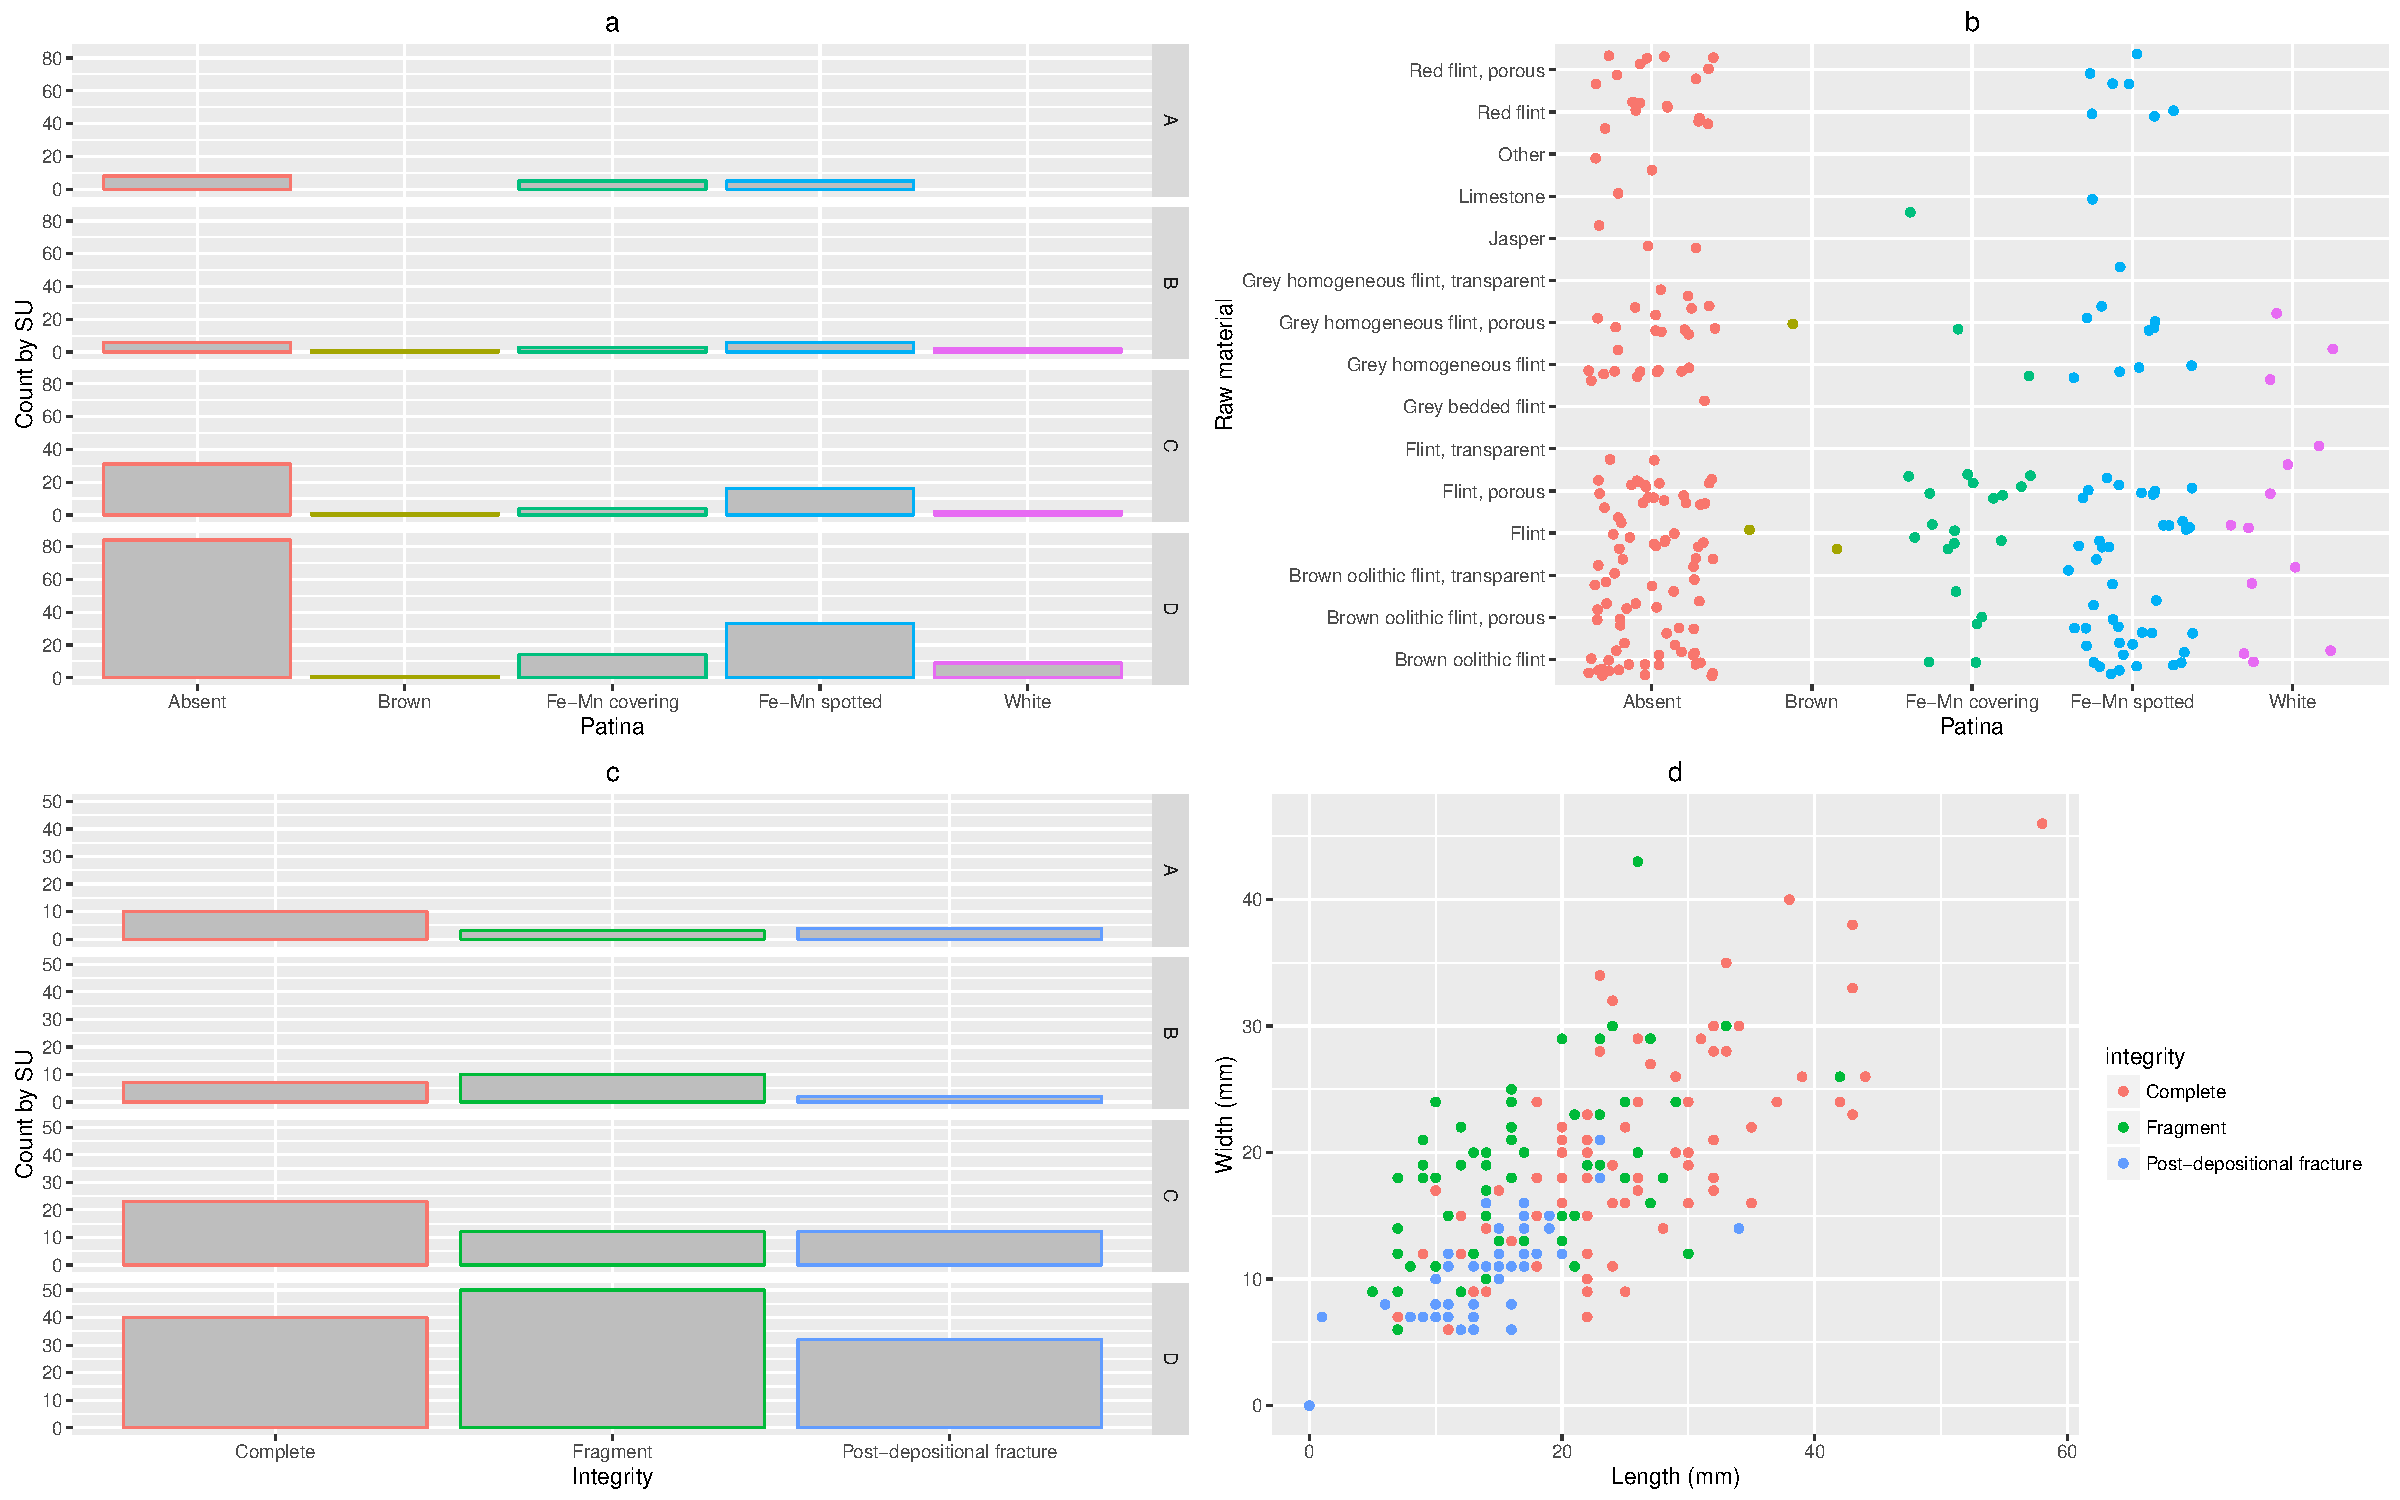
\includegraphics[width=1\textwidth]{../artwork/Fig2.pdf}
  \caption{Frequency of patinae on the lithic assemblage (a) and their distribution on raw materials (b); frequency of fractures (c); scatterplot of artifact dimensions (d).}
  \label{fig:2}
\end{figure}

\section{Spatial data collection and sampling}

Since 2007, systematic field investigations of the P13 fissure have been carried out by the University of Ferrara (in collaboration with the Universities of Torino and Roma Sapienza, until 2010).

From the first excavation season, a grid of $1$ square meter units has been set. Since 2010, the three-dimensional coordinates of the finds are recorded with a Total Station, which replaced the use of a water level. Orientation (dip and strike) of coordinated faunal remains (length $\geq2$~cm), geological clasts (length $\geq5$~cm) and all the lithic artifacts is estimated with a $45$ degree of accuracy, which is not precise enough for detailed fabric analysis.

In order to avoid possible sampling issues in spatial data analysis due to the variation in the recording methods, we select subsets of the lithic and faunal collection, excluding SU's A and B, because they have been excavated prior the use of the Total Station.

Focusing on SU's C and D, we scale the windows of analysis according to the extension of excavated areas for each SU, excluding the presence of the large blocks of rock. We reduce in this way the impact of the Modifiable Area Unit Problem (MAUP) in point pattern analysis \citep{Openshaw1996}, especially insidious in this study due to the particular geological setting of the site. The analyzed areas of SU's C and D are respectively $4.34~m^{2}$ and $5.82~m^{2}$.

During 6 years of excavations, more than $1600$ of $2152$ macro vertebrate fossils have been spatially recorded: $471$ from SU C and $916$ from SU D. However, \citet{Bagnus2011} conducted taphonomical analysis on fossils recovered during the 2007 to 2010 field seasons and only $593$ of these are classified in one of the three taphorecords (Tab.~\ref{tab:1}). Our sample includes $135$ coordinated elements of the $282$ analyzed fossils from SU C. From the total number of $366$ lithic artifacts collected until the 2014 field season, $147$ have been recorded with three-dimensional coordinates. Our sample includes $34$ lithics from SU C and $84$ from SU D. From the micro mammal assemblage, we include in this study only the \emph{Allophaiomys ruffoi} species. Of the $53$ arvicoline teeth collected from the screen-washed sediments, $49$ have secure provenance attribution from SU B ($n=2$), C ($n=14$) and D ($n=33$) \citep{Lopez-Garcia2015}. However, the \emph{A.~ruffoi} point pattern does not represent the exact distribution of the remains. Indeed, we randomly displaced ($r=0.5$) each point indicating the provenience of the sieved sediment.

\section{Vertical distribution}

The vertical distribution of finds is a key factor in the analysis of site formation processes. Many processes can be well approximated by a ‘nearly’ normal distribution. However, testing the appropriateness of this assumption is an essential step in spatial data analysis. Strongly right skewed distribution would occur in case of a non-uniform vertical distribution of finds; thus requiring the analysis to acknowledge the covariate effect of gravity in the observed spatial pattern.

The vertical distribution of finds within SU C is globally unimodal, roughly simmetric (slightly left skewed), in spite of some outliers (Fig.~\ref{fig:3}a). It ‘nearly’ approximates the maximum-likelihood fitting of a normal curve (red line) with mean ($\mu$) = $-1.53$~m and standard deviation ($\sigma$) = $0.27$~m. However the Shapiro-Wilk normality test reject the null hypothesis of a gaussian distribution ($p-value=0.0005213$). On the other hand, the Q-Q plot (Fig.~\ref{fig:3}b) shows deviations from the theoretical normal distribution (red line) between one ($68.27\%$ of the sample) and two ($95.45\%$) standard deviations from the mean. The S-shaped empirical distribution recalls its left skew.

The global vertical distribution of finds resemble that of the faunal assemblage, due to the weight of the latter on the sample data ($n=471$). The distribution of the lithic artifacts is more left skewed, while the small sample of micromammals follows a multimodal distribution with a prominent peaks at $-1.2$~m (Fig.~\ref{fig:3}a). Although the difference in size of the two samples, it is worth notice that the mean value of the vertical distribution of the \emph{A. ruffoi} species is very close to that of the lithic artifacts (Welch Two Sample t-test $p-value=0.5803$).

The vertical distribution of finds in SU D is globally unimodal, slightly left skewed, with one peak at $-2.10$~m and no outliers (Fig.~\ref{fig:3}c). Although the distribution is close to the best fitting normal curve (red line) with $\mu=-2.34$~m and $\sigma=0.33$~m, the Shapiro-Wilk test rejects the hypothesis of normality ($p-value=2.497e-12$). The Q-Q plot (Fig.~\ref{fig:3}d) shows a more dispersed distribution respect to the former one. Its steepper line follows the theoretical normal distribution within one standard deviation from the mean ($68.27\%$ of the sample).

Compared with the global distribution, the vertical distribution of lithic artifatcs slightly skews to the right. Nevertheless, the Shapiro-Wilk test fails to reject the normality hypothesis ($p-value=0.2742$). On the other hand, the micromammals distribution is multimodal and slightly shifted to the right (Fig.~\ref{fig:3}c). Its mean ($-2.284$~m) is quite close to the mean of the lithic sample ($-2.423$~m). However, the Welch t-test rejects the hypothesis of two equal sample means ($p-value=0.01414$). If we cannot state that the two distributions have the same mean, we remark the highest density of both the assemblages at around $-2.5$~m.

\begin{figure}
  \centering
  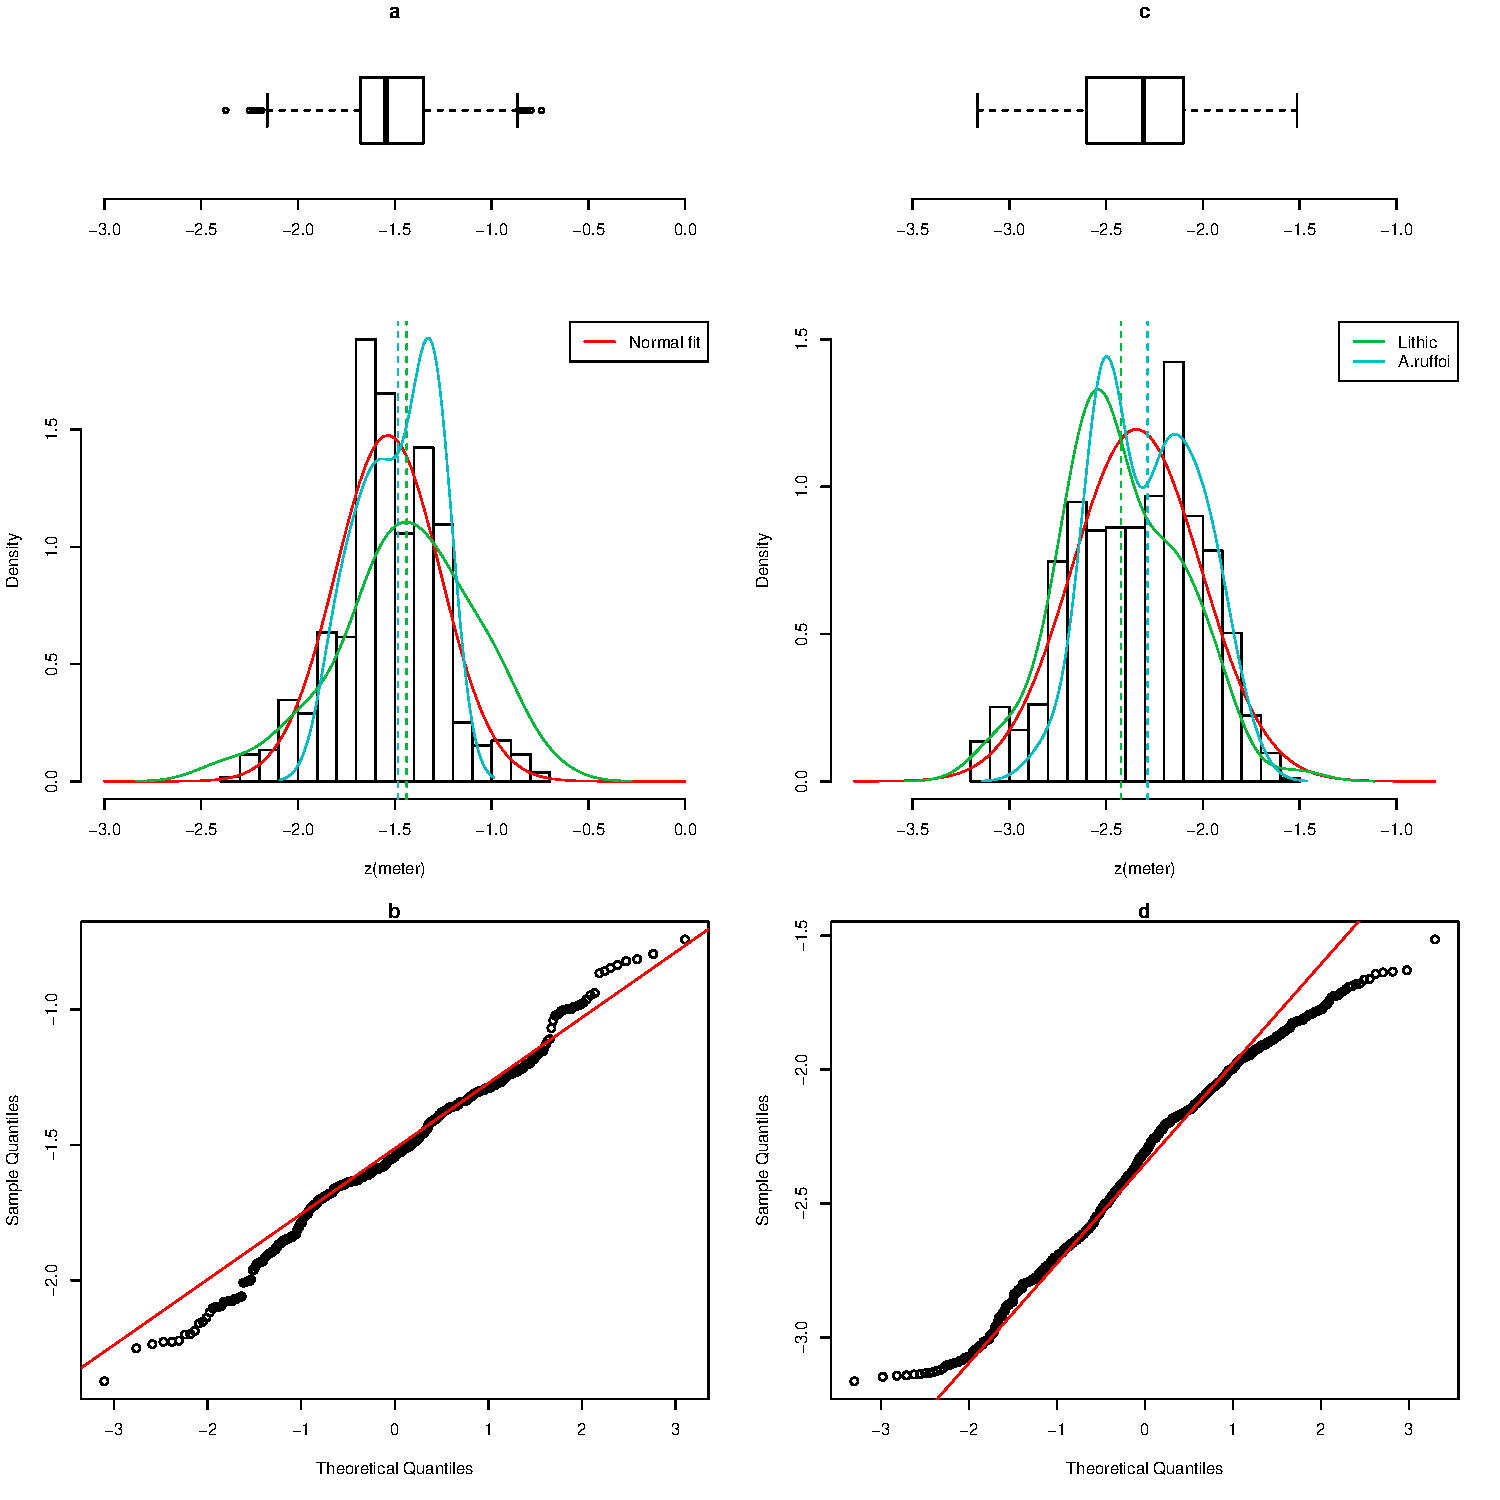
\includegraphics[width=1\textwidth]{../artwork/Fig3.pdf}
  \caption{Vertical distribution of finds in SU's C (a,b) and D (c,d).}
  \label{fig:3}
\end{figure}

As for the vertical distribution of the identified taphonomic features on the lithic and faunal assemblages, figures~\ref{fig:4}a,b illustrate the overall distribution of patinae on the lithic artifacts, across SU's C and D. The histogram shows the increasing number of finds between the two sedimentary units. This trend is reflected as well in the rise of Fe-Mn patinated artifacts ($41\%$ in SU C and $45\%$ in SU D), compared to non-patinated ones (respectively $50\%$ and $48\%$). The kernel density estimation (blue and green lines) shows a slightly higher occurrence of patinated artifacts at the lower part of the sequence (below $-2.5$~m), whereas in SU C (up to $-2$~m) there is no evident preference in the vertical distribution of patinae. The higher density of patinated artifacts, linked to the concentration of lithics observed in figure~\ref{fig:3}c at about $-2.5$~m, can be localized in a restricted spot at the bottom right corner of the excavated area (Fig.~\ref{fig:4}a).

Restricting the analysis to SU C, the vertical distribution of coordinated macro vertebrate fossils analized by \cite{Bagnus2011} spans $71\%$ of the elevation range of the complete assemblage from the same SU. However, beeing only the $29\%$ of the population, we acknowledge that our sample cannot be considered representative.

The densities of the low and medium rate of oxides resemble the general distribution (Fig.~\ref{fig:4}c,b). Low values follow a ‘nearly’ normal distribution (Shapiro-Wilk normality test $p-values=0.2186$). The density of high oxidized remains ($54\%$ of the sample) draws a left skewed distribution, with a peak at about $-1.3$~m; whereas fossils with a medium degree of oxides are skewed to the right. However there is no clear preference for oxides to occur deeper in the sequence. The mean values are very close to each other and lower values of oxides are more dense at the bottom of the SU.

As for the distribution of the three taphorecords, the prominent peak of TR1 at $-1.6$~m (Fig.~\ref{fig:4}f) contrast with a more distribuited and mixed distribution of the second and third group of fossils. However, the very low frequency of TR1 ($n=9$) limits further analyses.

\begin{figure}
  \centering
  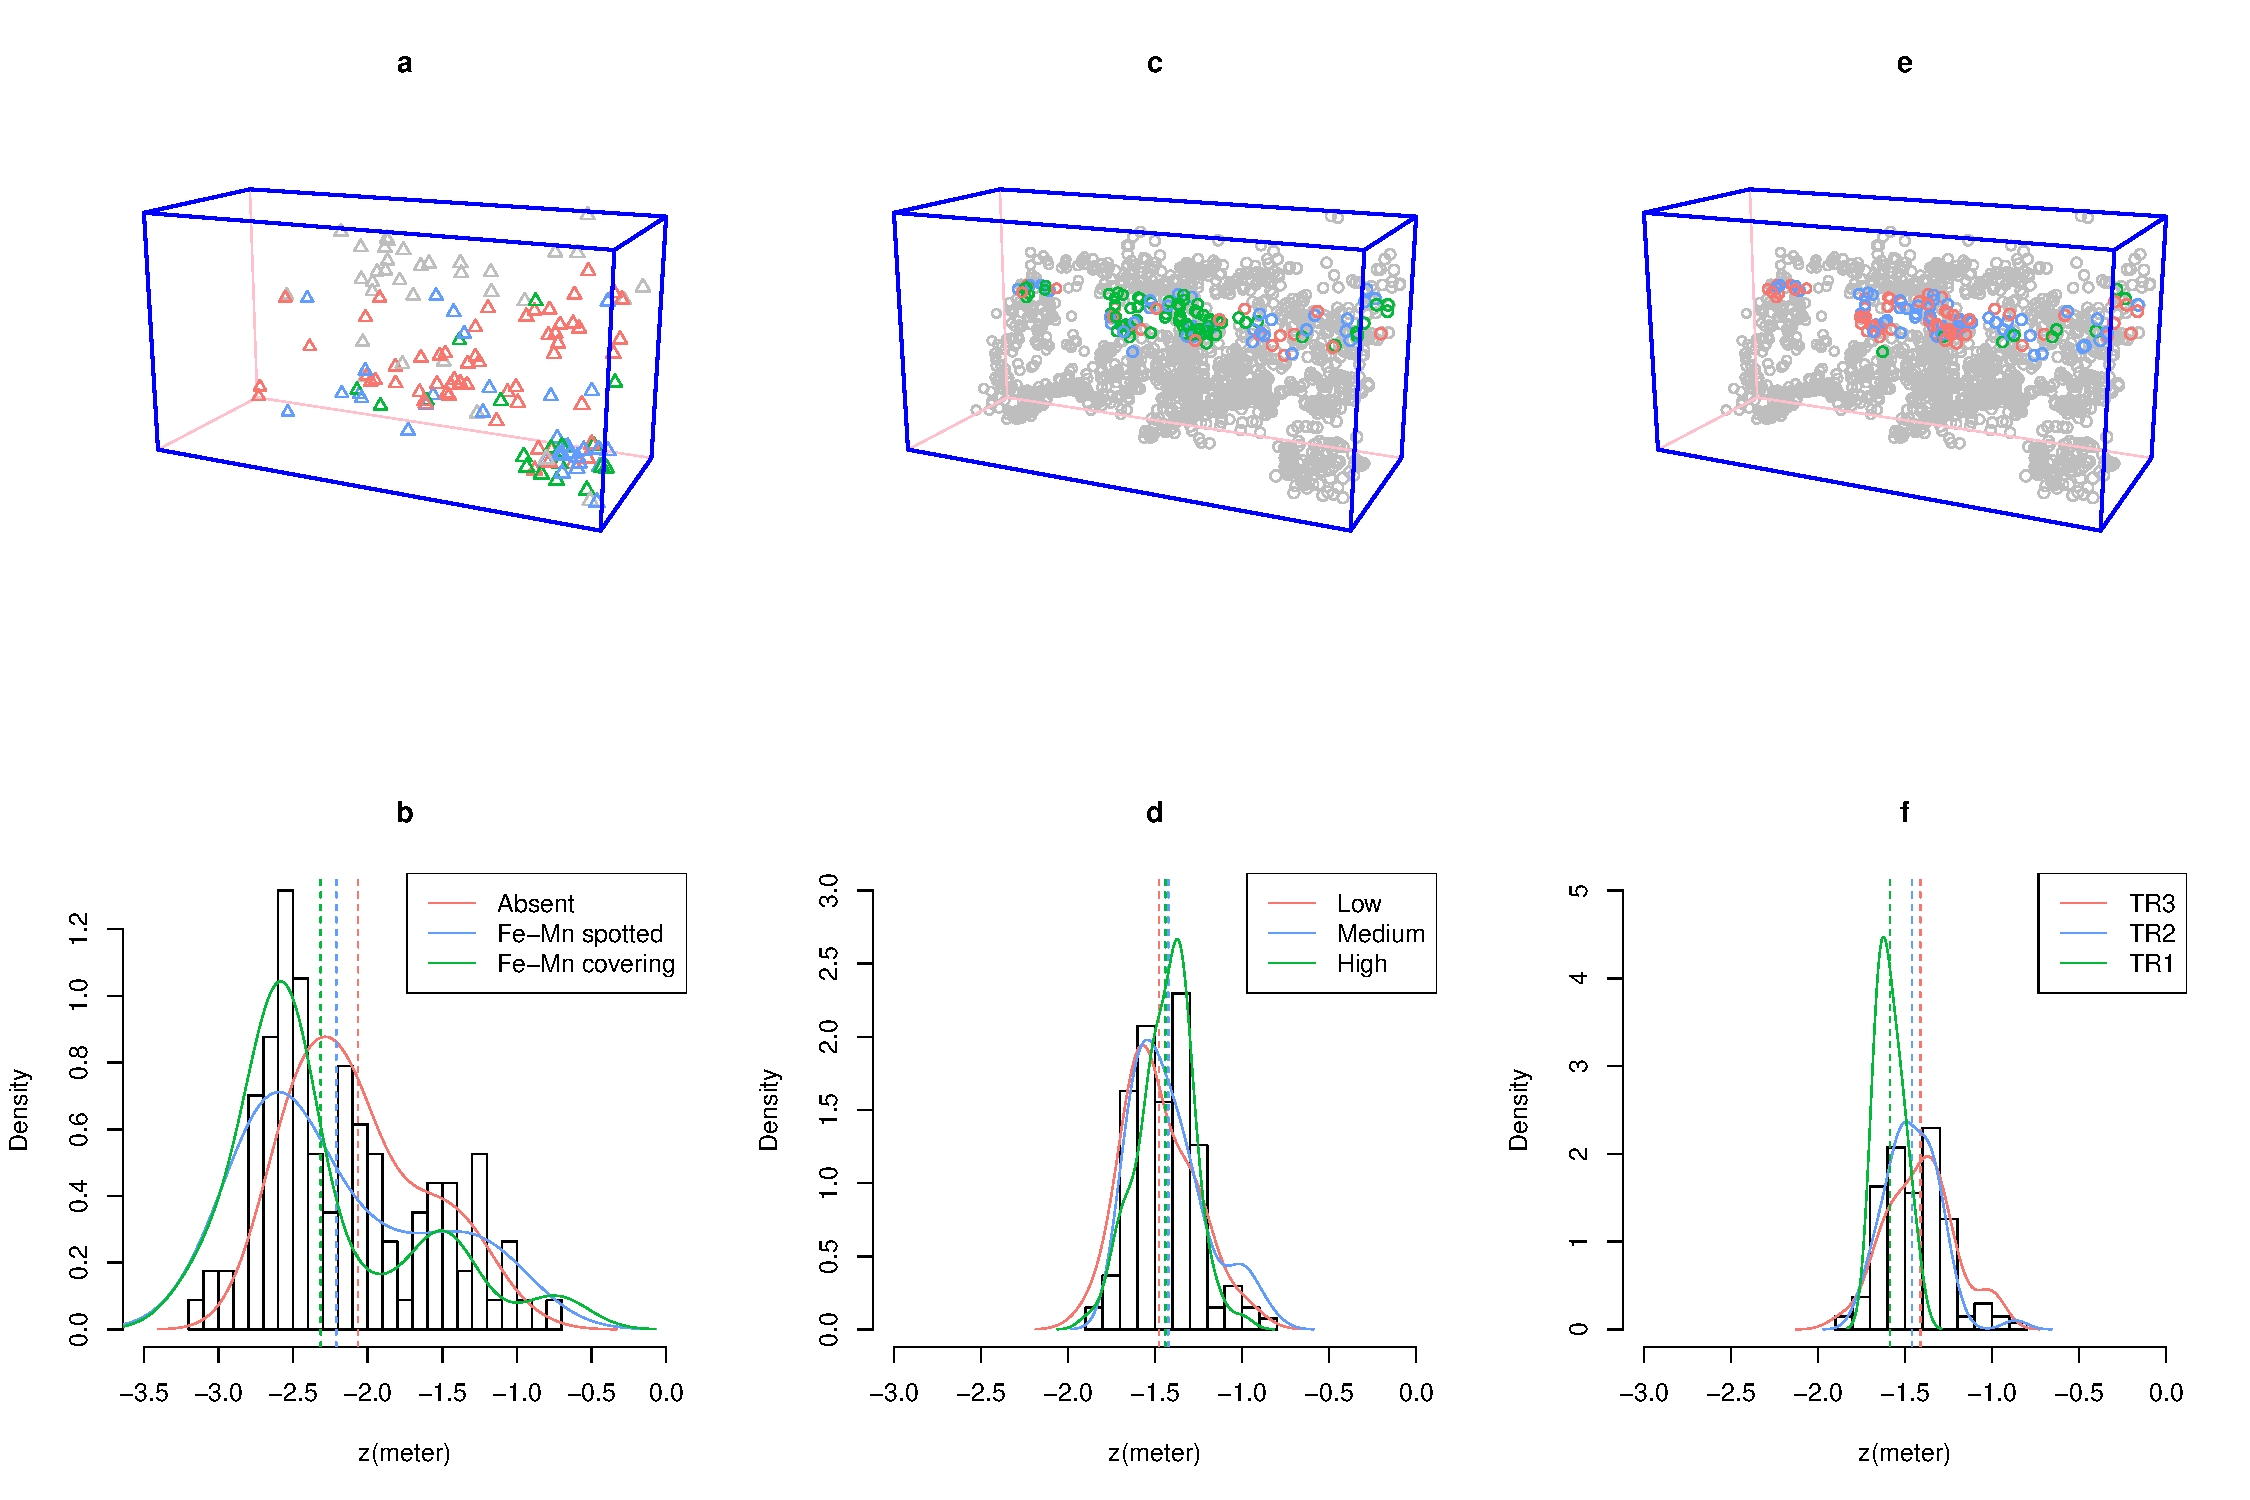
\includegraphics[width=1\textwidth]{../artwork/Fig4.pdf}
  \caption{3D and vertical distributions of Fe-Mn patinae on the lithic assemblage from SU's C and D (a,b); oxides (c,d) and taphorecords (e,f) from the faunal sample.}
  \label{fig:4}
\end{figure}

Although our study is constrained by the small sample of fossils and by its limited spatial extension to SU C, the analysis of the vertical distribution of Fe-Mn oxides in the faunal and lithic assemblages does not show any clear global pattern. Indeed, even taking into account the localized cluster of artifacts at the very bottom of SU D (Fig.~\ref{fig:4}a), the process responsible for the distribution of Fe-Mn oxides seams to operate indistinctly through the complete stratigraphic sequence, with no explicit preference for lower elevations.

With no evidence for strong right skewed distributions of finds in SU's C and D, we have reasons to exclude the covariate effect of gravity in the observed spatial pattern. The subsequent point pattern analyses are directed to the study of the 2D spatial distribution of fossils, lithics and their taphonomic status.

\section{Point pattern analysis}

The observed patterns of the archaeological and paleontological remains within SU's C and D, as well as the patterns of taphonomic features recognized on them, have been treated as realizations of spatial point processes, i.e. site formation and modification processes.

Indeed, a spatial point pattern is generally defined as the location of events generated by a point process, operating simultaneously at different scales: a first-order global scale and a second-order local scale \citep{Bailey1995}. The former results from the frequency (density) of events within a bounded region; the latter results from spatial dependency between points, e.g. from a tendency for values of the process at nearby locations to interact with each other. Three different types of interpoint interaction are possible: random (or Poisson); regular and cluster. Regular patterns are assumed to be the result of inhibition processes, while cluster patterns are the result of attraction processes. Therefore, two main issues of interest are explored by spatial point pattern analyses: the distribution (density) of entities in space and the existence of possible interactions between them \citep{Ord1972}.

First-order effect in the observed point-pattern is generally non-parametrically evaluated by means of kernel density estimation \citep{Diggle1985}. As an average density of points in the study region, intensity informs about uniform or inhomogeneous distribution of events.

Multiple scales of second-order patterning and the probability of a stochastic occurrence are explored by the Ripley's $K$ summary function \citep{Ripley1976,Ripley1977} and derivates, for both univariate and bivariate point patterns. The $K$ function is designed to identify the relative aggregation and segregation of point data at different scales. The univariate $K(r)$ function measures the expected number of events found up to a given distance $r$ around an arbitrary event. By comparing the estimated value $\hat{K}(r)$ to its theoretical Complete Spatial Randomness (CSR) value, it is possible to assess what kind of interaction exists between events. The bivariate function, or cross-type $K_{ij}(r)$ function seeks to evaluate, at each distance $r$, the spatial relation between two types $ij$ of observed events. In this case, the definition of the null hypothesis uses a randomization technique of either the location of one of the types (random shift hypothesis), or the type itself of the event at each point, preserving the original location (random labeling hypothesis) \citep{Goreaud2003}. The former aims to evaluate the spatial relationship between patterns of two independent processes, while the latter assumes the same process in determining the pattern for different types.

Especially in small dataset, the estimation of correlations between points is biased by edge effects, arising from the unobservability of points outside the window of analysis. In order to reduse that bias, we implement here Ripley's isotropic edge correction \citep{Ripley1988,Ohser1983}.

Monte Carlo simulations \citep{Robert2004} are used to generate pointwise critical envelopes of random expected values for the null hypotheses, providing an adequate level of statistical significance. We choose a small significance level ($\alpha=0.01$ obtained with $199$ simulations), due to the higher possibility to commit a Type 1 error by testing our hypotheses. Values of the empirical distribution (black solid line) are plotted against the theoretical Poisson distribution (red dotted line) and the simulated global envelope of significance (grey area). For $K(r)$, when the solid line of the observed distribution is above or below the shaded grey area, the pattern is significantly clustered (points are closer together than would be expected for a complete random pattern) or dispersed. For $K_{ij}(r)$, the benchmark value $\pi r^2$ is consistent with independence between the points of type $i$ and $j$, and does not imply a Poisson distribution.

\subsection{Formation processes}

In order to investigate the processes involved in the formation of the Pirro Nord deposit, we provisionally assume the deposition of each sedimentary unit to be the result of mass wasting events filling the fissure and resulting in the distribution of fossils and artifacts independently of each other.

To test the appropriateness of our working assumption, we first analyse the overall distributions of finds, treated as univariate point patterns. Applying a set of exploratory statistics, we aim to determine the nature of the depositional processes, e.g. if they raise in- or homogeneous distributions. Then, we analyse the relative patterns of the faunal and lithic assemblages from SU's C and D. In this case, we treat the two distributions as multitype point patterns.

The intensity of the lithic and faunal assemblages is non-parametrically estimated by first performing a Gaussian smoothing kernel of their distributions, for both SU's. Likelihood cross-validation bandwidth, which assumes an inhomogeneous process, is selected for each pattern. Edge correction is applied using the method of \cite{Diggle1985}. Then, Berman's $Z_2$ test is used to determine whether or not the intensity depends on a spatial covariate $Z$, assuming that the spatially varying (inhomogeneous) intensity is a function of $Z$. Thus, in order to measure the strength of dependence on the covariate, we use the Receiver Operating Characteristic (ROC) curve. Spatially adaptive smoothing, nearest-neighbour density and scan tests have been used in order to assess for the evidence of hot sposts in the intesities of the unmarked point patterns. Estimations of the $K(r)$ and the Kaplan-Meier corrected empty-space $F(r)$ functions provide further methods for the interpretation of the distributions.

Multitype summary functions are used in the analysis of the dependence between points of the two assemblages. In this case, our main research question is whether different types of finds have the same spatial distribution. The cross-type $K_{ij}(r)$ function and the Kaplan-Meier corrected nearest-neighbour $G_{ij}(r)$ function are used to estimate the association between points of type $i$ and $j$, for any pair of types of finds. Positive spatial correlation between the two types of finds whould suggest that lithic artifacts are more likely to be found close to fossils than would be expected for the hypothesis of \emph{independence}. It would confirm the field observations about their close stratigraphic association and further support our hypothesis that both patterns are the realization of one depositional process. On the other hand, segregation of the two patterns is equivalent to variation in the probability distribution of types. Segregation could be interpreted as the expression of preferential/differential depositional processes. In this case, more detailed analyses would be necessary.

\subsection{Post-depositional processes}

In order to evaluate the degree of post-depositional disturbance of the deposit, the spatial dependence of observed taphonomic features is assumed to be the expression of a related diagenetic process. Measured phenomena that are closer together in space, tend to be more related than those further apart \citep{Tobler1970}.

Like in applications of point pattern analysis in spatial epidemiology \citep{Diggle2003,Gatrell1996}, we distinguish between \emph{cases} and \emph{controls}. The distribution of cases of a certain taphonomic alteration can be regarded as the realization of a diagenetic point process, whereas controls points refer to non-altered remains. In a conditional analysis of a spatial case-control study the locations are fixed covariates, and the taphonomic status is treated as a random variable. The simplest null model (\emph{random labelling}) is that the taphomonic status of each find is random, independent and with constant risk of occurrence.

Spatial correlations of diagenetic alterations on the lithic and faunal assemblage are explored by the $K_{ij}(r)$ function, random labelling the pair case/control of Fe-Mn oxidation. We assume in this case that an independent process (karst water circulation), subsequent to the initial event responsible for the accumulation of the finds in each SU, determined their preservation status. Positive deviations from the null hypothesis, suggest that cases are more likely to be found close to controls than would be expected if their status was randomly determinated. On the other hand, negative deviations would indicate segregation between cases and controls. Thus, it would suggest that the action of post-depositional water-related processes could have locally reworked the original distribution, determining the altered status of the remains.

All the spatial analyses were performed using the \emph{spatstat} package \citep{Baddeley2015} in \textsf{R} statistical software \citep{RCoreTeam2015}.

A repository containing a compendium of data, source code and text is archived at the DOI:

\section{Results}

\subsection{Formation processes}

Figures~\ref{fig:5}c,d show the smoothing kernel estimation of the faunal assemblage intensity respectively in SU's C and D. Lithic artifacts and micromammals remains of the \emph{A.~ruffoi} species are superimposed on it. The visual assessment of the plot suggests positive spatial association between the three types of finds. Higher intensities in the distributions are evident at specific values of the \emph{x} coordinate ($6<x<7$ and $8<x<9$), in both the sedimentary units. Yet, a concentration of artifacts, already observed in figure~\ref{fig:3}c and \ref{fig:4}a,b, is evident at the lower right corner of SU D (Fig.~\ref{fig:5}e). Such higher densities of finds are clearly showed as well in the scatterplots of the projected third coordinate (Fig.~\ref{fig:5}a,b). Notably, the thickness of the sedimentary unit cannot be accounted to be responsible for those hot spots with higher density of finds. Neither the apparent inhomogeneous intensities along the $x$ axes is supported by the ROC curves (Fig.~\ref{fig:5}e,f). Even if Bermans's $Z_2$ tests suggest significant evidence of dependence on the $x$ covariate, the ROC curves show that it does not have strong disctiminatory power.

\begin{figure}
  \centering
  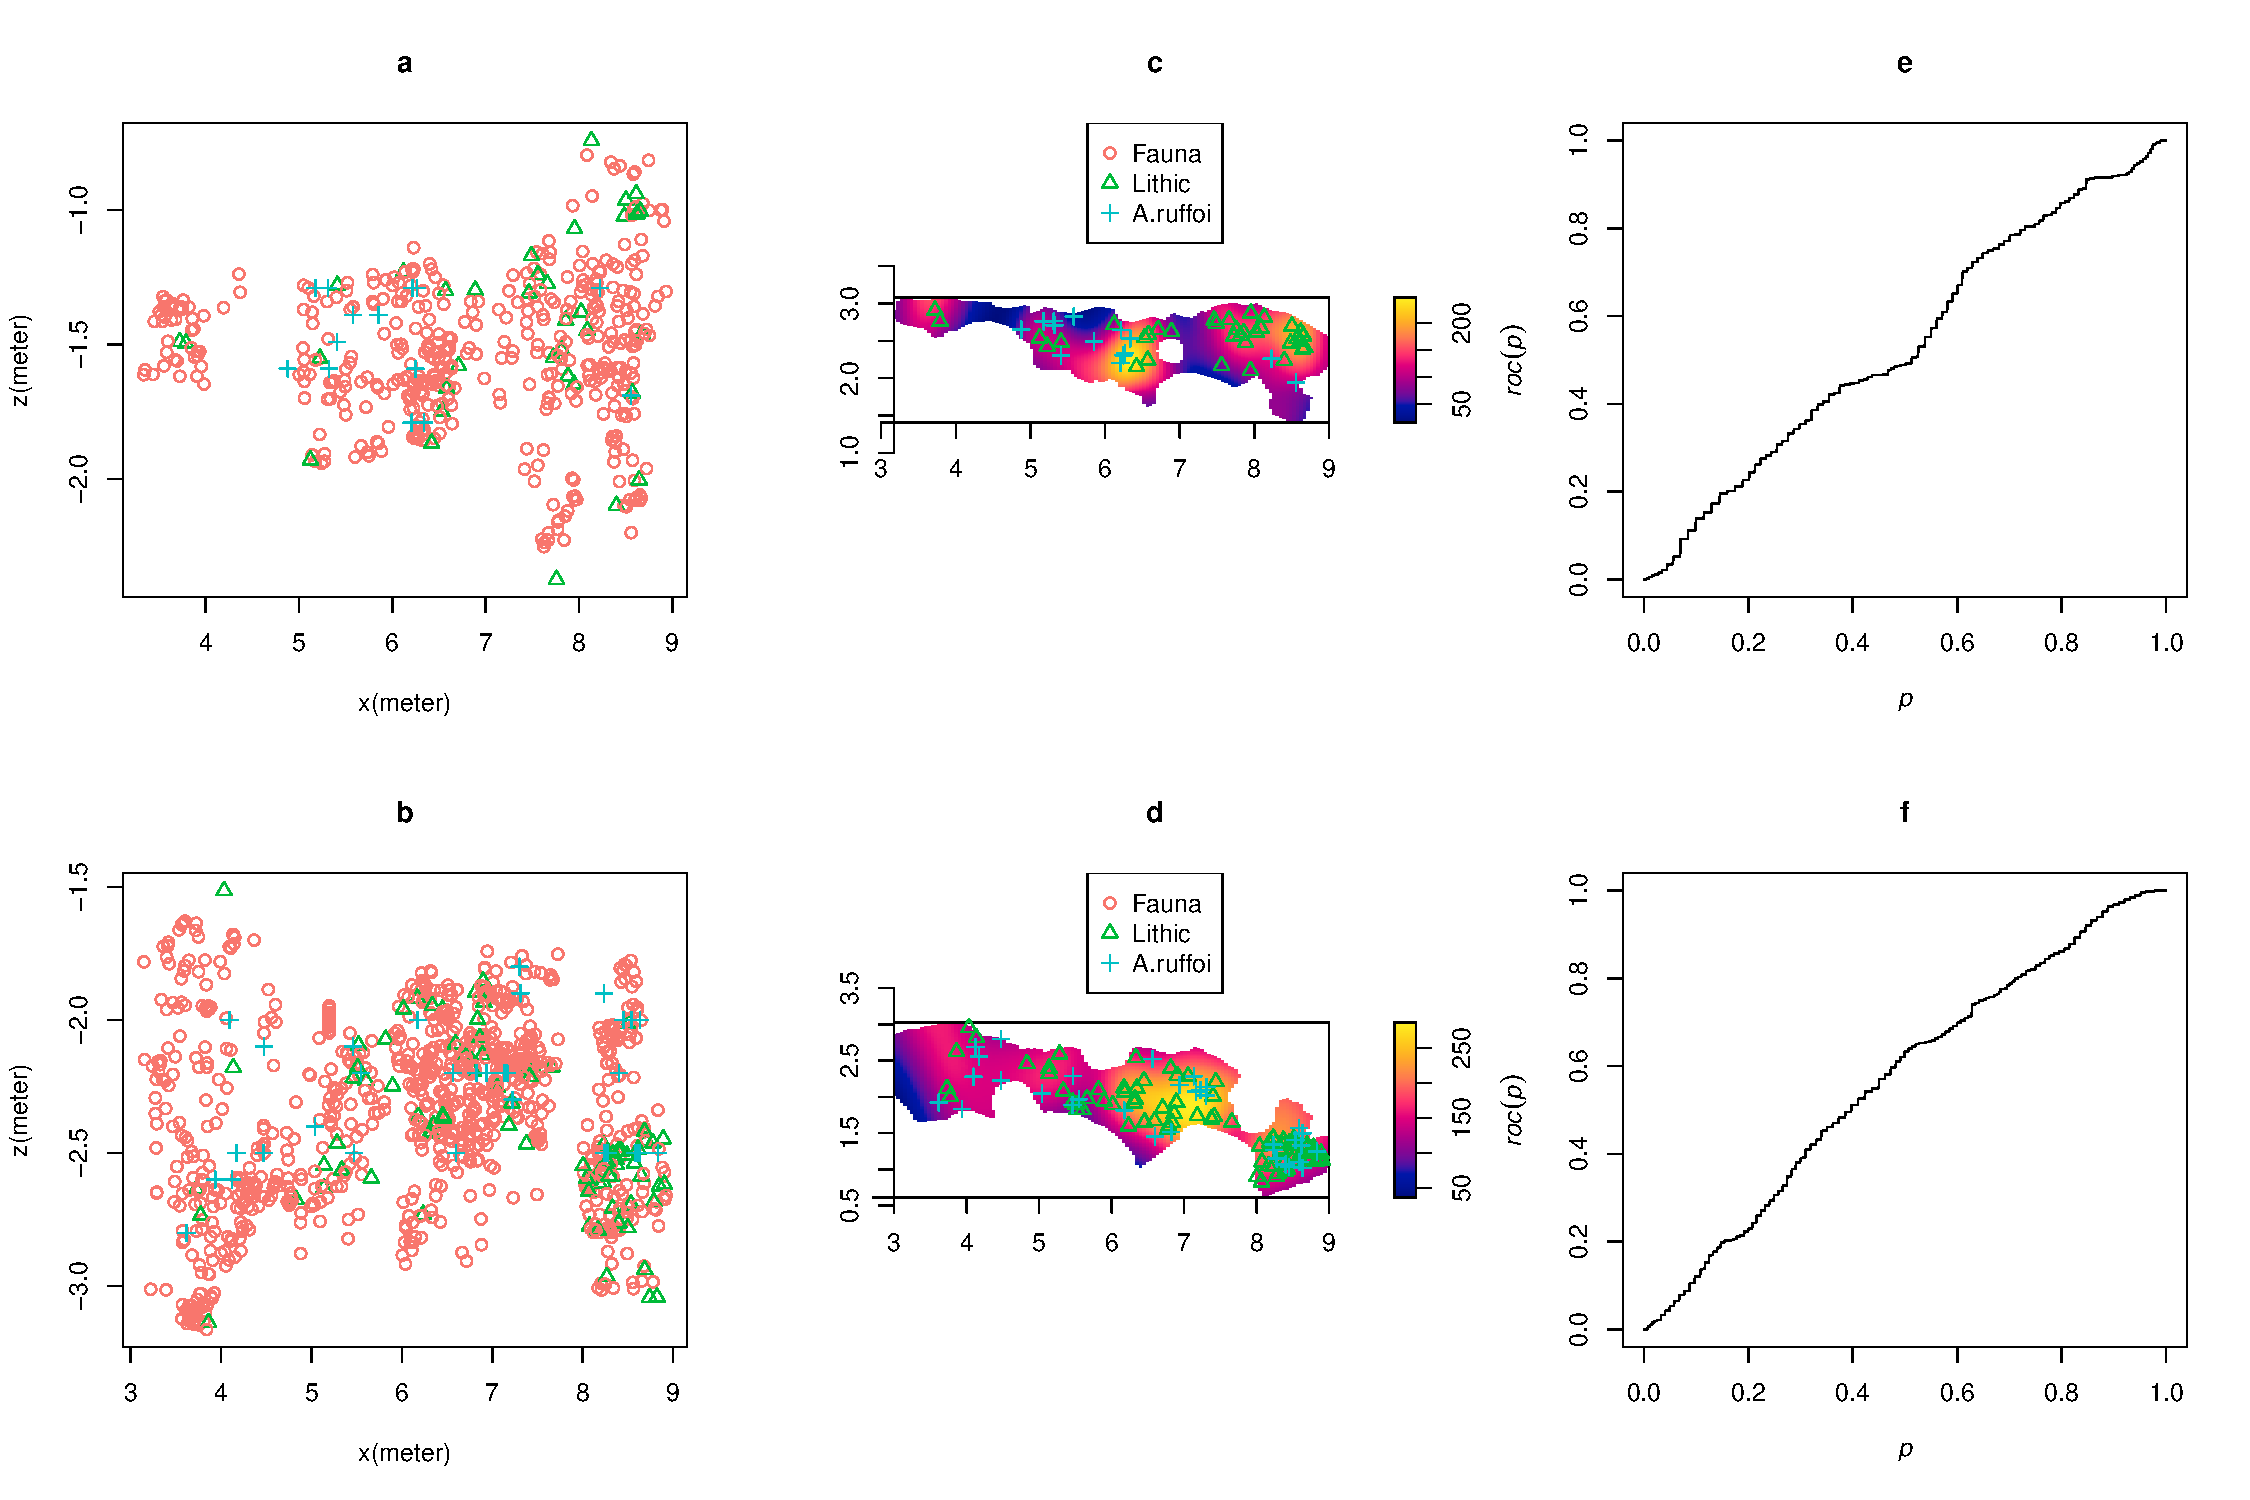
\includegraphics[width=1\textwidth]{../artwork/Fig5.pdf}
  \caption{Scatterplot of finds from SU's C (a) and D (b); Smooth density estimation of the faunal assemblage and distribution of lithic artifacts and \emph{A.ruffoi} remains in SU's C (c) and D (d); ROC curves for the covariate $x$ coordinate in SU's C (e) and D (f).}
  \label{fig:5}
\end{figure}

Figures~\ref{fig:6}a,d show the resulting p-values of likelihood ratio scan test statistic. The test detects differences in the densities of the distributions, showing zones with high abundance of finds. The estimated homogeneous $\hat K(r)$ and $\hat F(r)$ functions are consistent with this result. For both SU's C (Fig.~\ref{fig:6}b,c) and D (Fig.~\ref{fig:6}e,f) they suggest strong deviation from the null hypothesis of CSR towards aggregation, at any scale.

\begin{figure}
  \centering
  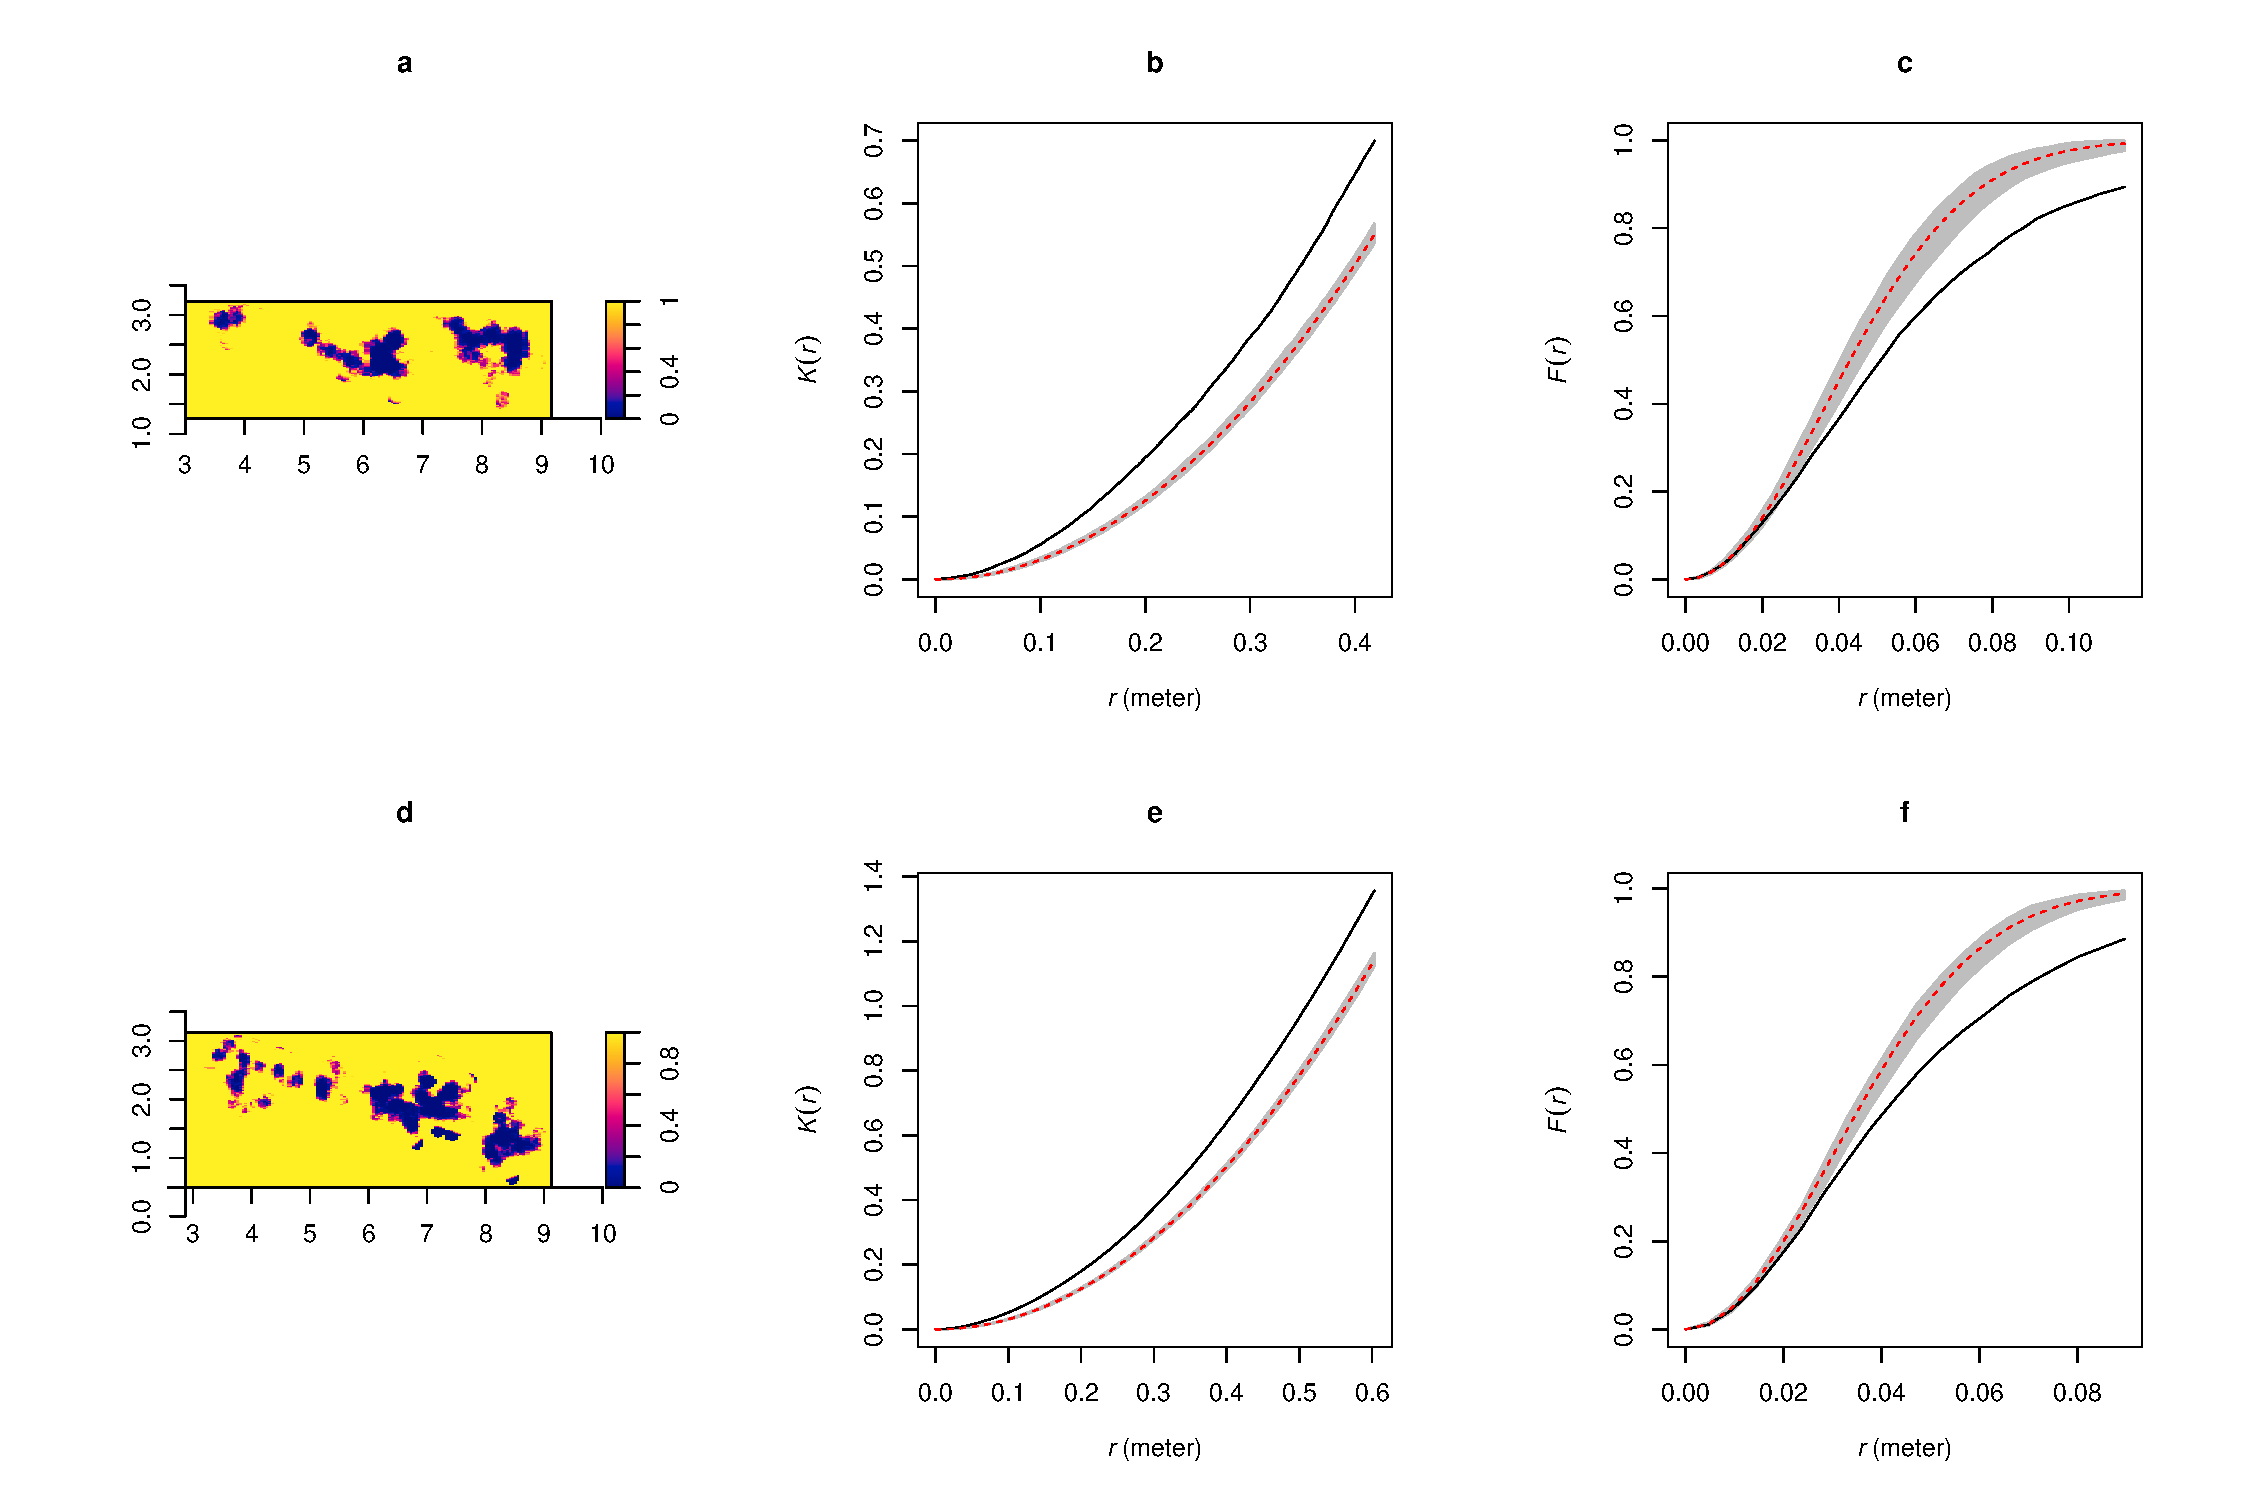
\includegraphics[width=1\textwidth]{../artwork/Fig6.pdf}
  \caption{p-values of the likelihood ratio scan test, with logarithmic colour scale, for SU's C (a) and D (d); pointwise envelopes of the homogeneous $K(r)$ and $F(r)$ functions for unmarked finds from SU's C (b,c) and D (e,f).}
  \label{fig:6}
\end{figure}

In analysing a point pattern, it is confounding and it may be impossible to distinguish between clustering and spatial inhomogeneity \citep{Baddeley2015}. Given the context of the site, and the results of our non-parametric analyses, we proceed considering the distributions of finds as the results of cluster homogeneous processes. The bivariate version of the homogeneous $K_{ij}(r)$ and $G_{ij}(r)$ function allow us to statistically test the hypothesis of aggregation between the types of remains.

In figure~\ref{fig:7}, the top line of panels (a,b,c) shows the ordinary estimations of the $K$ function for the three types of finds (Fauna, Lithic and \emph{A.~ruffoi}) from SU C. Panel~\ref{fig:7}a resembles figure~\ref{fig:6}b and indicates statistical significant clustering of the faunal remains for any values of $r$. The lithic assemblage shows as well a significant cluster tendency, for $r>0.1$, while it fails to reject the null hypothesis of CSR for lower values. Instead, the estimated $\hat{K}(r)$ for the micromammals shows aggregation, but, for all values of $r$, we cannot state that the distribution is not random. This result might reflect the random displacement applied to the micromammal point pattern.

The middle and bottom lines of panels in figures~\ref{fig:7} show estimations of the homogeneous cross-type $K$ and $G$ functions for all pairs of type $i$ and $j$. Interestingly, figure~\ref{fig:7}d suggests positive spatial correlation between lithic and faunal remains at any values of $r>0.05$. The corresponding $G_{ij}(r)$ function measured the cumulative distance from each point of type $i$ (Lithic) to the nearest point of type $j$ (Fauna). It shows (Fig.~\ref{fig:7}g) that the nearest-neighbour distances are significantly shorter than expected, but we cannot reject the hypothesis of independence between fossils and artifacts. However, the short scale of the function suggest that any artifacts is surrounded by fossils. This result statistically confirms the stratigraphic association of artifacts and fossils, previously based on field observations. On the other hand, deviations between the $\hat{K}_{ij}(r)$ function and the benchmark $\pi r^2$ suggest segregation between lithics and \emph{A. ruffoi} speciments, but the hypothesis of independence between the two types is more significant (Fig.~\ref{fig:7}e,h). Conversely, the small mammal assemblage is closer to the rest of the fossils than expected for independent distributions, for $r>0.2$. For lower values of $r$, the $K$ and $G$ functions fail to reject the hypothesis of independence.

\begin{figure}
  \centering
  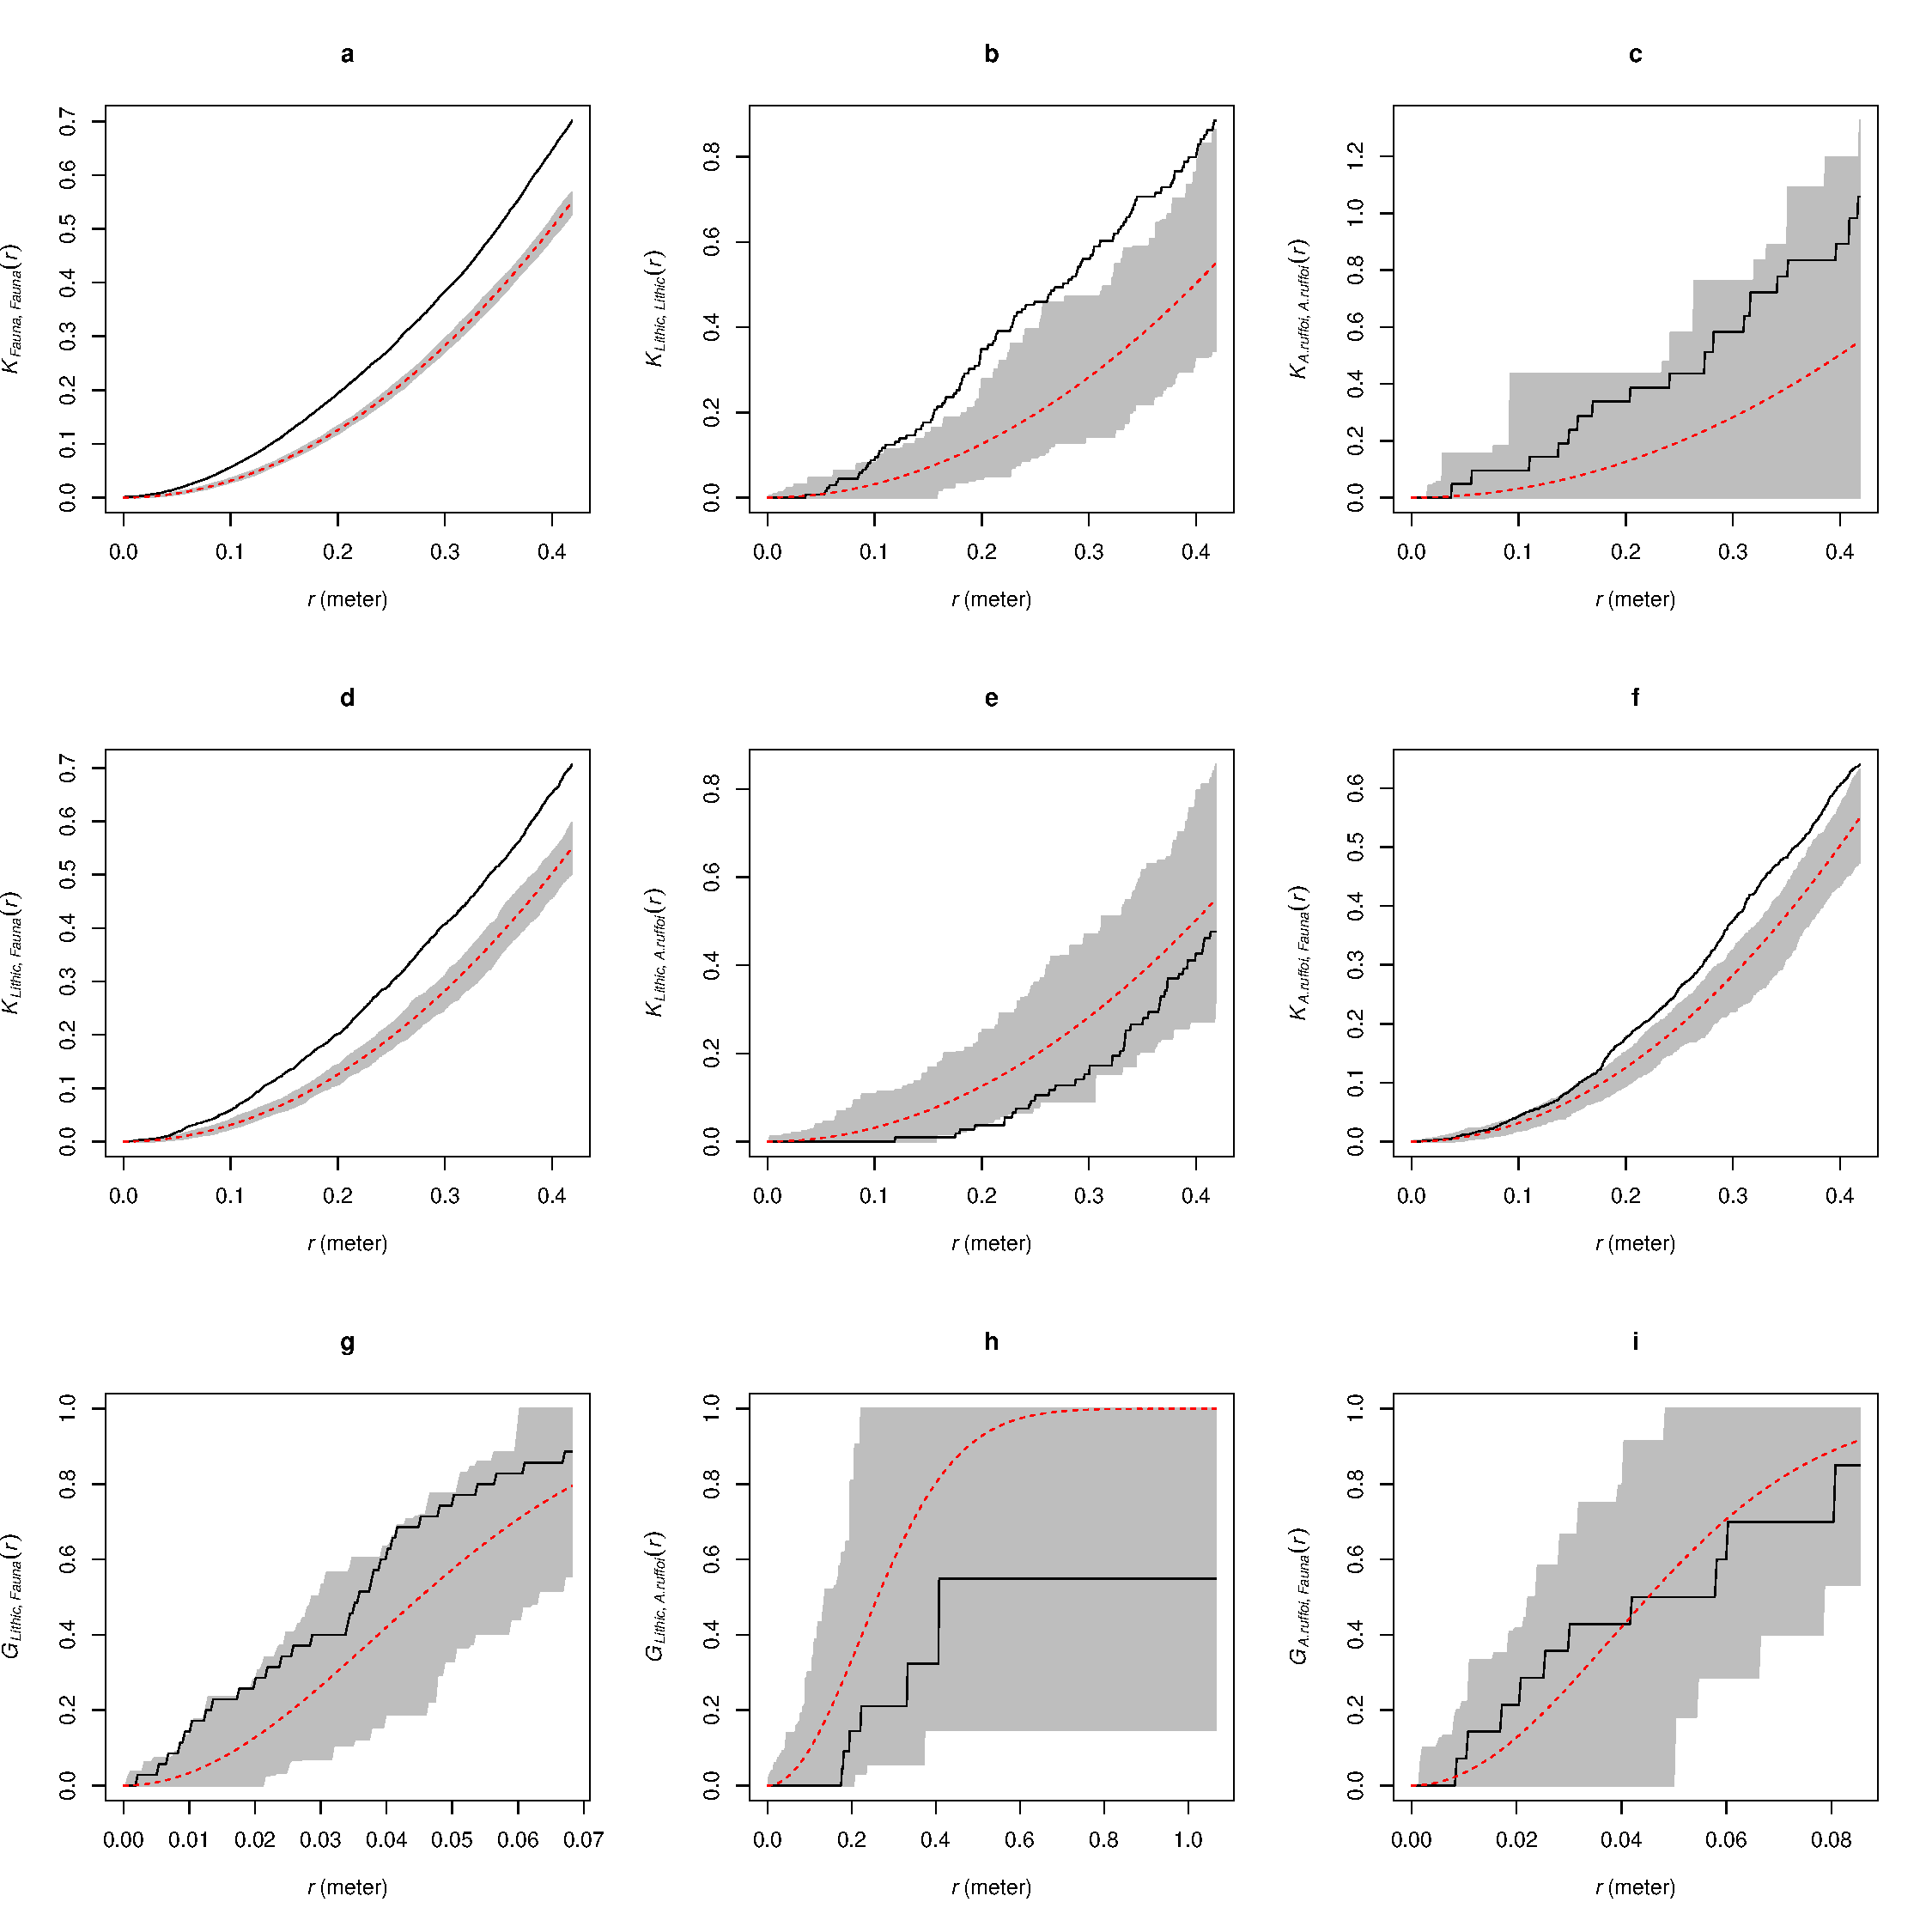
\includegraphics[width=1\textwidth]{../artwork/Fig7.pdf}
  \caption{Pointwise envelopes of the homogeneous cross-type $K_{ij}(r)$ and $G_{ij}(r)$ functions for all pair of type $i$ and $j$ in SU C.}
  \label{fig:7}
\end{figure}

The top line of panels in figure~\ref{fig:8} (a,b,c) shows estimations of the $K(r)$ function for the three types of finds from SU D. Panel~\ref{fig:8}a confirms the same clustering trend of the faunal assemblage. Analogous to the distribution of finds from SU C, the global pattern is mostly weigthed on the faunal assemblage (Fig.~\ref{fig:6}e). Conversely, in SU D the distribution of lithics shows stronger significant clustering for $r>0.1$. Again, the resulting $\hat{K}(r)$ for the micromammal assemblage suggests a statistically insignificant aggregation tendency for all values of $r$, but $0.4<r<0.5$. In contrast to the previous result, estimations of the $K_{ij}(r)$ function support significant positive correlation between the lithic artifacts and the \emph{A.~ruffoi} remains (Fig.~\ref{fig:8}e). Thus, they occur closer that expected in the case of independent distributions. Panel~\ref{fig:8}f shows the same positive correlation also between micro and macro mammals for $r>0.2$. The panels~\ref{fig:8}d,g show as well significant positive aggregation between lithics and fossils for values of $r>0.1$. In addiction, the estimated $\hat G_{ij}(r)$ function offers a closer view of the distribution. For values of $r<0.1$, it fails to reject the hypothesis of independence.

\begin{figure}
  \centering
  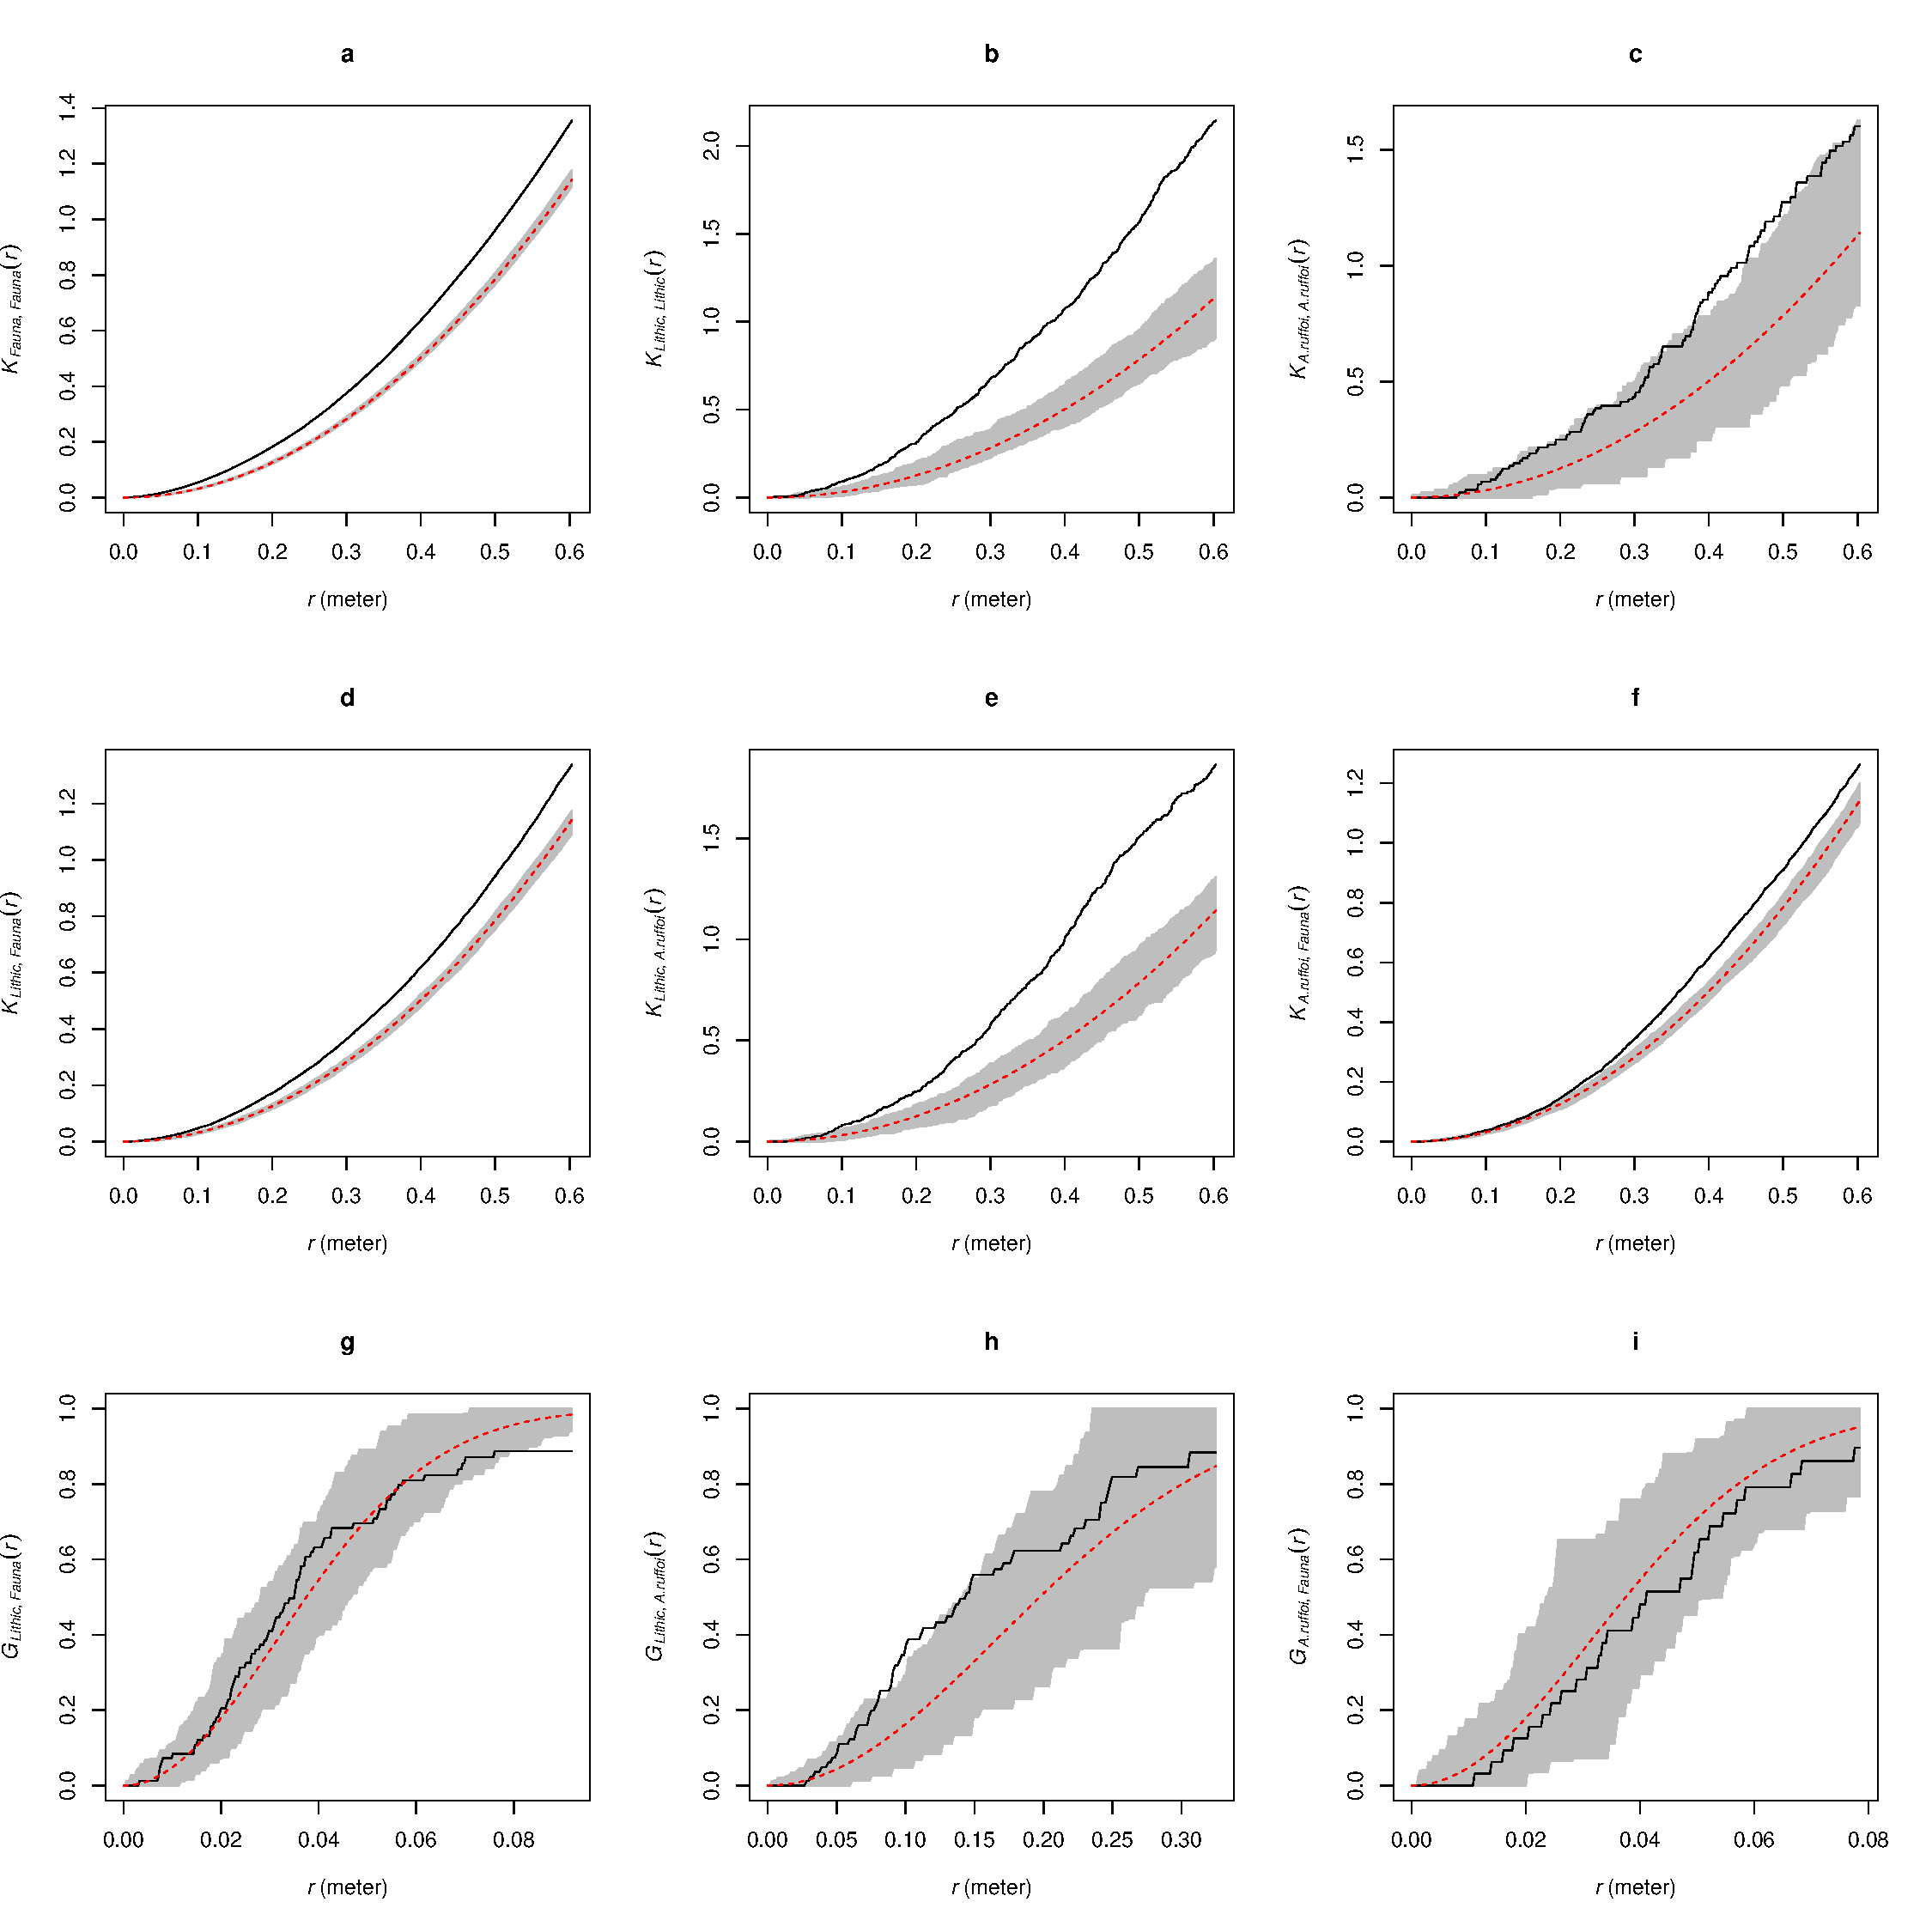
\includegraphics[width=1\textwidth]{../artwork/Fig8.pdf}
  \caption{Pointwise envelopes of the homogeneous cross-type $K_{ij}(r)$ and $G_{ij}(r)$ functions for all pair of type $i$ and $j$ in SU D.}
  \label{fig:8}
\end{figure}

\subsection{Post-depositional processes}

To achieve our second objective, namely to evaluate the degree of post-depositional disturbance of the deposit, we first analyzed spatial distribution of oxides on the lithic and faunal assemblages independently, then we moved to a comparative analysis. We are particularly interested in the spatial distribution of Fe-Mn oxides (cases) compared with the absence of them (controls).

Figure~\ref{fig:4}a does not suggest segregation of patinated and not-patinated lithics. If we perform random labeling of the presence of Fe-Mn (spotted and covering) with its absence in both the stratigraphic units, the outputs of the cross-type function (Fig.~\ref{fig:9}a,~b) show that the observed altered artifacts are, with a $0.01$ level of significance, randomly and independently located in SU C. The positive discrepancy between the estimated $\hat K_{ij}(r)$ and the benchmark $\pi r^2$ indicate aggregation of cases and controls, but it lies within the grey envelope of the \emph{random labeling} hypothesis. Conversely, patinated and non-patinated lithics in SU D appear to be closest to each other than expected for the null hypothesis. In this unit the observed $\hat K_{ij}(r)$ function over-exceeds the envelope at values of $r>0.4 m$, hence it indicates statistically significant aggregation. Such pattern statistically confirms the visual assessment of figure~\ref{fig:4}a. Consequently, oxidized and non-oxidized artifacts most probably occur in SU D well aggregated in space, while their aggregation is not statistically significant in the above unit.

We could not compare the oxidation patterns between lithics and fossils from SU D, because the taphonomic analysis of \citet{Bagnus2011} did not include fossils from this unit. Thus, we focused our analysis on SU C.

The distribution map (Fig.~\ref{fig:4}c) does not suggest any evident pattern. When we apply random labelling of the absence of oxidation with the medium and high degrees of its presence, the output of the bivariate $K_{ij}(r)$ function shows a segregation tendency between them, but it is not statistically significant. (Fig.~\ref{fig:9}c). A random and independent distribution of oxides is more plausible.

Finally, figure~\ref{fig:9}d shows the result of the $K_{ij}(r)$ function, random labeling the cases (medium and high degrees) and controls (absent or low degree) of Fe-Mn oxides on the lithic and faunal assemblages from SU C. The empirical values of the cross-type function are balanced on the theorerical expectation for complete spatial independence (red line). It clearly lies inside the grey envelope of significance. Therefore, our analysis shows an independent spatial distribution of Fe-Mn patinated and non-patinated lithic artifacts and fossils from SU C. In the lower unit (SU D), where figure \ref{fig:4}b indicates higher density of oxidized artifacts, estimations of the cross-type $K$ function suggests that they occur closer than expected to fresh ones.

\begin{figure}
  \centering
  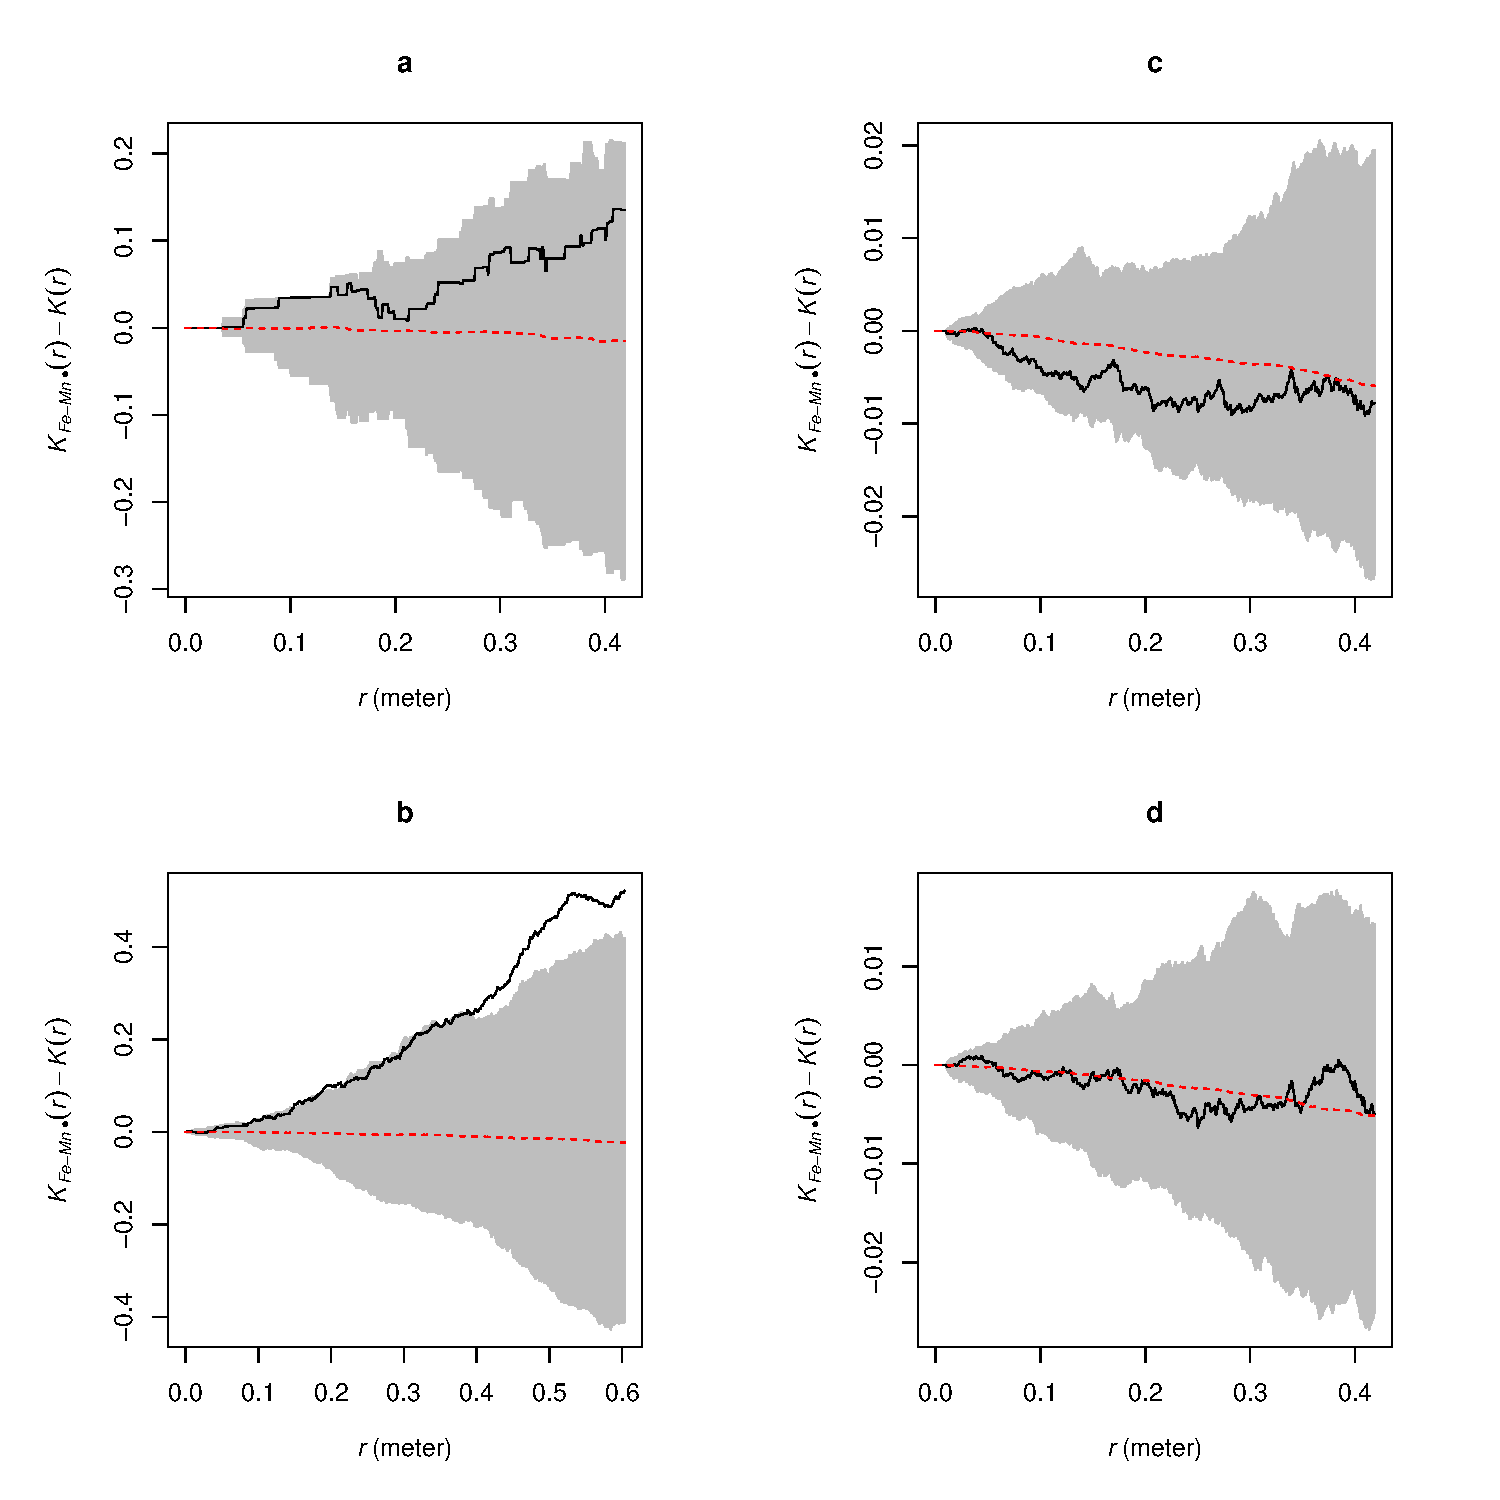
\includegraphics[width=1\textwidth]{../artwork/Fig9.pdf}
  \caption{Pointwise envelopes of the homogeneous bivariate $K_{ij}(r)$ function, random labeling \emph{cases}/\emph{controls} of patinated lithics in SU's C (a) and D (b); oxidated fossils in SU C (c); Fe-Mn oxids on the lithic and the faunal assemblage from SU C (d).}
  \label{fig:9}
\end{figure}

\section{Discussion}

The Early Pleistocene site of Pirro~Nord (fissure P13) has yielded evidence for one of the earliest occurrences of hominins in Europe. The importance of the evidence calls for a multivariate taphonomic analysis in order to establish the nature of the processes involved in the formation of the deposit and the degree of its post-depositional disturbance. We address that need by investigating the spatial association of the archaeological and paleontological remains, as well as the spatial distribution of artifacts and fossils with diagenetic alterations. We focused our analysis on the lower stratigraphic units C and D, since they provide the most significant corpus of finds and they have been studied with the same research protocol.

\subsection{Formation processes}

Non-parametric analyses have been carried out in order to characterize the processes responsible for the formation of the deposit. Then, we accounted for the relative spatial pattern of the different types of finds.

The vertical distribution of the archaeological and paleontological assemblages does not appear to be affected by strong gravitational effects. On the other hand, it resemble a 'nearly' normal distribution and suggests a very close mean occurence of lithic artifacts and \emph{A. ruffoi} remains, despite the small sample of micromammals (Fig.~\ref{fig:3}). A visual interpretation of the projected third coordinate (Fig.~\ref{fig:5}a,b) also suggests that the intensity of finds is not a function of the covariate $z$. Moreover, higher densities are not linked to the thickness of the stratigraphic units. They are clearly localized at values of $6<x<7$ and $8<x<9$ in both the SU's, as showed also by figures \ref{fig:5}c,d and \ref{fig:6}a,d. Indeed, the Berman's $Z_2$ test for the dependence of the point process on the spatial covariate $x$ failed to reject the null hypothesis for SU C ($p-value=0.00445$) and D ($p-value=1.913e-14$). However, even if it suggests significant evidence that the intensity depends on some covariate, the effect of that covariate could still be weak. ROC curves (Fig.~\ref{fig:5}e,f) indicate that the $x$ coordinate does not have disciminatory power.

\cite{Bartlett1963} showed that it is possible to formulate a point pattern which can be equally interpreted as a Poisson inhomogeneous process, or a homogeneous cluster process. According to our non-parametric analyses, we proceeded under the assumption that the processes involved in the formation of the Pirro Nord (P13) deposit are homogeneous and clustered. The scan tests in figures \ref{fig:6}a,d show hot spots of points, mostly localized between $6<x<7$ and $8<x<9$. The cluster correlation between all the finds is significantly confirmed by the estimations of the $K$ and $F$ functions (Fig.~\ref{fig:6}). The first lines of panels in figures \ref{fig:7} and \ref{fig:8} offer a type-based view of these patterns. Indeed, the estimated $\hat K(r)$ functions of the faunal assemblage (Fig.~\ref{fig:7}a and \ref{fig:8}a), which constitute the bigger part of the analyzed sample of data, resemble the results for the complete populations (Fig.~\ref{fig:6}b,e). The lithic assemblage also show significat aggregation; while the small sample of \emph{A. ruffoi} falls inside the envelope of CSR.

Faunal remains and lithic artifacts show some overlapping when evaluated by means of Gaussian smoothing kernel (Fig.~\ref{fig:5}c,d). Positive spatial association between fossils and lithics is statistically confirmed by the cross-type $K$  and $G$ functions for the examinated SU's (Fig.~\ref{fig:7} and \ref{fig:8}). Fossils and artifacts tend then to occur aggregated with each other (they are closest than expected for a independent process). Significant spatial proximity is also showed between artifacts and micromammal remains, especially in SU D.

According to the results of our analyses, the stratigraphic and spatial association between the types of remains should be considered as the result of the same formation process. Finds occur in the clayey-sand sediment together with a high number of angular to sub-rounded gravels and boulder-sized rock clasts. Such a stratigraphic setting suggests repeated mass-wasting processes (at least two events, represented by SU's C and D, which were included in this study) with low degree of reworking in a relatively short span of time \citep{Arzarello2012}. Rapid-moving and chaotic water-laden masses, such as mud-flows or earth-flows, of soilwash and rock rubble with fossils and artifacts \citep[p.~46]{Butzer1982}, could have been triggered by intense rainfalls and trapped in the karst sink-hole directly opening to the outside. Sedimentary filling would have derived from the top, by gravity, directed into the empty space between the large limestone blocks that made up the internal structure of the fissure. The thickness of the layers is likely correlated to the intensity of such events.

On the other hand, the clustered distribution of all the finds cannot be linked to the thickness of the statigraphic units. The big blocks of calcarenite, which in some places transect the stratigraphic units (Fig.~\ref{fig:1}), created a complex internal structure and might have influenced the direction of sediment accumulation. However, sedimentation rate, driven by the rugged topography of the site, does not seem to be spatially associated with the localized hot spots (Fig.~\ref{fig:6}a,d). Thus, clustering might have been a correlated effect of the formation process.

The presence of partially articulated vertebrate skeletal elements and their general low degree of weathering indicate fast burial and transport of bones from nearby locations \citep{Bagnus2011}. A close spatial proximity between the original location of the finds and the karst fissure, as well as a relatively fast burial, is also corroborated by the unrounded ridges and edges of the lithic artifacts and by the technological consistency of the assemblage \citep{Arzarello2014}.

In conclusion, our spatial statistics analyses confirm the field observations about the spatial association of archaeological and paleontological remains.

\subsection{Post-depositional processes}

After dealing with our first research question (to examine the spatial distribution of finds in the context of the site formation processes), our analyses were particularly directed to test the hypothesis of post-depositional processes reworking the deposit. We assume that the spatial aggregation of taphonomic surface alterations, and their relative segregation compared to non-altered finds, would indicate the localized activity of diagenetic agents.

We focused more on the spatial distribution of oxides, because traditional explanations for the development of Fe-Mn patinas on the surface of flint refer to the deposition of various iron and manganese oxides and hydroxides out of soil water \citep{Stapert1976}. Similarly, the origin of manganese coatings on fossils, in karst environments, may derive from circulating water, or from the manganese present in the surrounding limestone rock dissolved by groundwater \citep{Hill1982}.

The vertical distribution of oxides on the lithic artifacts and the sample of faunal remains (Fig.~\ref{fig:4}) spans the complete stratigraphic sequence and apparently shows a gradual increase through the lower layers, especially in the lithics assemblage. Intensity of oxides is indeed more likely proportional to the density of finds and not related to the depth.

By applying a set of spatial statistics (namely cross-type $K_{ij}(r)$ function) to the archaeological and paleontological remains, we searched for evidence of localized areas, which might have been subjected to the presence of water, especially water-flows.

In SU C, the spatial distribution of Fe-Mn patinas on lithics and fossils is, with a certain degree of significance, the result of independent processes (Fig.~\ref{fig:9}a,c,d). We cannot state that there is aggregation (spatial proximity) between oxidized finds and fresh ones. Neither the results of the bivariate $K$ function, random labeling the cases/controls of Fe-Mn coating, show segregation, which indicative of spatially defined diagenetic processes. In contrast, in SU D (Fig.~\ref{fig:9}b), patinated and fresh artifacts occur significantly spatially aggregated to each other for values of $r>0.4 m$. They occur closer than expected by an independent process at bigger scale. However, the pattern is, with a certain confidence level, independent.

\citet{Rottlander1975} identified a possible different cause of Fe-Mn coatings in the iron that is already present in the flint. In this light, the spatial association of flint artifacts with and without patination also depends on the chemical and microstructural composition of the raw material itself. On the other hand, the same oxides affecting a good percentage of finds, have been equally found broadly scattered on the numerous clasts of calcarenite that are included in the matrix, thus supporting an external origin of the Fe-Mn coating process.

The content of water and organic matter in the sedimentary body could be responsible for the randomly diffuse Fe-Mn patinations. In presence of organic matter, indeed, it is likely that the release of organic acids will accelerate patination on chert \citep{Burroni2002}. Moisture of the sedimentary body could also be accounted for the wide random spread of Fe-Mn coatings.

We did not find statistically significant evidence of aggregation of oxidized records compared to non-oxidized ones (Fig.~\ref{fig:9}c); thus, we can exclude the assumption of localized concentration of water, which is included in the hypothesis advanced by \citet{Bagnus2011} for the presence of inner flows reworking the deposit.

Due to the small sample size, we did not apply spatial analysis to the distribution of the three taphorecords. However, figure ~\ref{fig:4}e,f suggests that fossils from the TR1 group occur spatially aggregated with fossils from the TR2 and TR3 groups. Considering the distribution of Fe-Mn oxides on the lithic and faunal assemblages, the re-elaborated TR1 \citep[\emph{sensu}][]{Fernandez-Lopez1991,Fernandez-Lopez2007,Fernandez-Lopez2011} might not be associated with the reworking action of water-flows and might be more likely correlated to random and limited rearrangement of parts of the sedimentary matrix.

A possible cause of some localized movement of sediments could be the rock falls from the vault of the karst fissure, during the deposition of SU's C and D. As showed in figure~\ref{fig:1}, an abrupt increase in the number of boulder-sized rocks is observed within the lower layers. Moreover, rock falls caused most of the post-depositional fractures on the faunal assemblage \citep{Bagnus2011}. Such intense erosional process could most likely be correlated to the seismic activity of the region \citep{Bertok2013}.

Results of our analyses suggest that post-depositional taphonomic alterations occured with a certain significance as result of independent processes. However, keeping a caution approach to spatial analysis, a documented point pattern can be most realistically thought of as the result of multiple processes heterogeneously working at different scales \citep{Bevan2013}. Multiple or repeated post-depositional processes could obliterate contemporaneous or preceding patterns, resulting in a final random distribution of the record.

Moreover, karst site formation processes are highly dependent on the structure and extension of the overall karsic system, as well on the surrounding environment. The lack of information about the original characteristics of the system and the reduced area of excavation strongly limit the analysis.

Furthermore, although the need for considering three dimensional distributions in site formation processes study, spatial point pattern statistics are at the moment not fully equipped to analyze three-dimensional patterns, especially when the study-area corresponds to a three-dimensional volume with a complex shape such as a karsic structure.

On the other hand, "one must look to non-spatial evidence to corroborate or disprove theories about spatial processes" \citep[p.~8]{Hodder1976}. The integration with other taphonomic disciplines reinforces the results of spatial analyses and outline new opportunities for point pattern analyses. As recently remarked \citep{Cobo-Sanchez2014}, taphonomic research should be multivariate \citep{Dominguez-Rodrigo2010} and it should include spatial analysis as a heuristic tool in the interpretation of site integrity. This is especially demanding when the research questions deal with past human behaviour and even more so when site dating is based on the stratigraphic association of artifacts and fossils.

\section{Conclusions}

The Early Pleistocene site of Pirro~Nord~13 provides evidence of the earliest human presence in Western Europe. Lithic artifacts have been found in a karst fissure filling, together with late Villafranchian/early Biharian paleontological remains.

The main goals of our study were:
\begin{enumerate}
  \item to investigate the depositional processes involved in the formation of the deposit and
  \item to assess the degree of any potential post-depositional reworking of the archaeological and paleontological remains.
\end{enumerate}

The integration of spatial point pattern analyses with previous taphonomic studies on the faunal and lithic assemblages allowed us to test different hypotheses of site formation and modification processes.

On the basis of our analyses,
\begin{enumerate}
  \item we consider the deposit as the result of subsequent events of some type of mass-wasting process, such as a mud-flow or earth-flow, carrying rock rubble with fossils and artifacts. The applied set of spatial analyses confirm, with an adequate level of statistical significance, this assumption, based on field observations, regarding the spatial association between the finds.
  \item Based on our taphonomic point pattern analyses of several diagenetic features on the lithic and faunal assemblages, we reject the hypothesis of a substantial post-depositional reworking and mixture of the sedimentary deposit and we corroborate the stratigraphic integrity of the Pirro Nord 13 site.
\end{enumerate}

Finally, the present study answers the need for a taphonomic perspective in spatial analysis, by applying well developed quantitative methods in spatial statistics. Point pattern analysis can be very flexible and useful in the investigation of both cultural and taphonomic processes. Until now it has found limited application on taphonomic studies, but, as our study demonstrates, it offers new analytical opportunities to the multidisciplinary study of the complex processes that operate in the formation and modification of archaeological sites. It allows analysts to test multiscalar patterns and to model the taphonomic processes underlying archaeological distributions, which are otherwise difficult to identify from the simple visualization of maps, especially for those sites characterized by complex geo-stratigraphic settings.

\section*{Acknowledgements}

DG was supported by the European Research Council Starting Grant PaGE, No. 283503.

Fieldworks were financially supported by the University of Ferrara and the Apricena Municipality. Excavations were possible thanks to the concession by the Soprintendenza Archeologica della Puglia and Ministero dei Beni e delle Attività Culturali; and thanks to the collaboration of Dott.ssa Anna Maria Tunzi. Excavations were also possible thanks to the kind disposability of Gaetano and Franco dell'Erba.

We would like to thank all those who attended the excavation campaigns for their indispensable cooperation; Julie Arnaud for her contribution to the 3D modeling of the site; Nick Thompson for English proofreading.

We are grateful to Vangelis Tourloukis and two anonimous reviewers for critical discussions and many constructive comments that helped to improve this manuscript.

\section*{References}

\bibliographystyle{elsarticle-harv}
\bibliography{pirronord_rr}

\end{document}
